\documentclass[12pt]{article}
\linespread{1.2}
\setlength{\parskip}{1em}
\usepackage{hyperref}
\usepackage{xpatch}
\usepackage[sorting=none]{biblatex}
\usepackage{fancyhdr}
\usepackage{float}
\usepackage{graphicx}
\usepackage[a4paper, margin=1.25in]{geometry}
\usepackage{makecell}
\addbibresource{references.bib}
\hypersetup{
    colorlinks=true,
    linkcolor=black,
    filecolor=magenta,      
    urlcolor=black,
    citecolor=black
    }
\urlstyle{same}

\title{}
\date{June 2025}

% Here you can find a backup of this project: 
% https://github.com/ThisisShoo/APS-1034-Team-Project-Report

% Lucid Chart: 
% https://lucid.app/lucidchart/4e7d9b66-8e03-4d3c-bbfb-40a45487144a/edit?viewport_loc=-784%2C-1980%2C6596%2C3320%2C0_0&invitationId=inv_5fac3005-5c65-482d-b08d-a74f334d73be

% System Dynamics Diagram:
% https://lucid.app/lucidchart/65582136-6a59-4926-a426-46b7bcc25d2a/edit?beaconFlowId=780B4308C833DFC5&invitationId=inv_41acb568-f723-4ad7-8733-0793af84f316&page=0_0#

% Drive Doc = https://docs.google.com/document/d/1SqCwM1th-N_Kp87VMr64HIsHCJK0QRoMJO3AX74vI7E/edit?usp=sharing

% https://docs.google.com/presentation/d/1pT7ffI62jmMRrgCiUe4Wh-LL00AeIwDbWfsZ_iKLuhs/edit?usp=sharing

%Links for the timeline: 
%\href{https://www.cbc.ca/news/canada/sudbury/elliot-lake-mall-chronology-from-birth-to-death-and-beyond-1.2799462}{https://www.cbc.ca/news/canada/sudbury/elliot-lake-mall-chronology-from-birth-to-death-and-beyond-1.2799462}

% https://globalnews.ca/news/402886/timeline-the-elliot-lake-mall-collapse/

% https://www.youtube.com/watch?v=2tO1L3SKhfU

% Link for the presentation slides:
% https://docs.google.com/presentation/d/1pT7ffI62jmMRrgCiUe4Wh-LL00AeIwDbWfsZ_iKLuhs/edit?usp=sharing

\begin{document}
\title{Causal Analysis based on Systems Theory (CAST) of the Algo Centre Mall Collapse}
\author{Teresa Sabu (1011567038), \\
Raul Martinez (1004821838), \\
Shuhan Zheng (1007136154), \\
Wenxuan Meng (1005434246), \\
Zhaoheng Li (1011349612), \\
Julian Lebenhaft (Instructor)
}
\maketitle

\newpage

\begin{table}[H]
    \centering
    \caption{Contributions of Team Members}
    \vspace{1em}
    \begin{tabular}[H]{|l|l|}
        \hline
        Tasks/Sections & Main Contributors \\ \hline
        \makecell{Formatting, review, \\ rewrite for tone (when applicable)} & Shuhan \\ \hline
        Executive Summary & Shuhan \\ \hline
        Introduction & \makecell{Shuhan (History \& CAST intro),\\ Raul (Timeline)} \\ \hline
        Step 1 - Assemble Basic Information & Teresa \\ \hline
        \makecell{Step 2 - Hierarchical Safety Control \\ Structure (diagram)} & Teresa / Raul \\ \hline
        \makecell{Step 2 - Hierarchical Safety Control \\ Structure} & Teresa \\ \hline
        \makecell{Step 2 - Hierarchical Safety Control \\ Structure (at time of accident)} & Teresa \\ \hline
        Step 3 - Bottom-up Analysis & Wenxuan \\ \hline
        \makecell{Step 4 - Top-down Analysis, GAP \\ Analysis} & Raul \\ \hline
        Step 5 - System Dynamics Model & Teresa \\ \hline
        Step 6 - Discussion/Recommendations & Zhaoheng \\ \hline
        Presentation & \makecell{Zhaoheng (lead \& review) \\ everyone else (their own sections)} \\ \hline    \end{tabular}
    \label{Contributions}
\end{table}

\newpage
\tableofcontents
\newpage

\section*{Executive Summary}
% Purpose: Summarize the objectives, key findings, and recommendations of the analysis.

% Overview: Provide a brief description of the Algo Centre Mall collapse, including the date, location, and immediate consequences.

\addcontentsline{toc}{section}{Introduction}
\section*{Introduction} 
% Author: Shuhan Zheng 
% Reviewer: Teresa Sabu

The Algo Centre Mall, located in Elliot Lake, Ontario, was constructed between 1979 and 1980 by Algocen Realty Holdings Ltd. Housing a public library, a government service center, a hotel and retirement residence, and various retail stores, the mall served not only as a commercial hub but also as a community gathering space. The three-story structure was composed of concrete and steel-reinforced concrete slabs supported by a steel frame, sitting on a sloped terrain facing northeast. A parking deck was built on the roof, which was accessible via ramps along the hillside. The parking deck was supported by a steel frame held together by bolted and welded connections, with a layer of hollow core concrete slabs on top. In 2012, a section of the roof deck collapsed after a long history of water leaks, structural deterioration, and, most importantly, neglect, resulting in the deaths of two people and over twenty injuries. This report aims to analyze the Algo Centre Mall collapse using the CAST (Causal Analysis based on System Theory) methodology, which focuses on understanding the systemic factors that contributed to the incident. The following section first provides a relatively brief history of the Algo Centre Mall and its deteriorating conditions leading up to the collapse, then gives an overview of the CAST methodology, and finally outlines the structure of this report.

\addcontentsline{toc}{subsection}{History of the Algo Centre Mall}
\subsection*{History of the Algo Centre Mall}

\addcontentsline{toc}{subsubsection}{Algocen built a defective mall amid a mining rush, sold its problems away at the sight of an economic downturn}

\subsubsection*{Algocen built a defective mall amid a mining rush, sold its problems away at the sight of an economic downturn}

Throughout the years that immediately followed its construction, the mall was plagued by significant structural issues, particularly with water leaks from the rooftop parking deck, owing to failed waterproofing measures. Such water leaks, along with cracks that developed in the concrete slabs, were reported as early as 1981, and the building's condition continued to deteriorate over the years. Ten years later, a report prepared by Trow Consulting Engineers Ltd. found that although the rooftop parking deck was generally in good condition, various components of the building had visible signs of deterioration, including the aftermath of failed repairs, sections of broken concrete, and surface rust on exposed steel. In the Report of the Elliot Lake Commission of Inquiry (henceforth referred to as the Elliot Lake Report) \cite{AlgoLakeReport1}, it was noted that the proposed waterproofing for the rooftop parking deck only met the requirements of the Ontario Building Code at that time on a technicality, for the 1975 code never specified what the waterproof membrane should be made of. Although a waterproof sealant was relied upon to act as a waterproofing membrane, it clearly failed to do so, as water leaks continued to be reported throughout the years. 

The aforementioned 1991 Trow report also indicated an abnormal amount of chloride content in the slabs, presumably from the de-icing salts used on the parking deck or brought in by vehicles, which proved to have exacerbated the corrosion of the steel components. Trow recommended the installation of a new waterproof membrane and a layer of asphalt to replace the existing concrete topping, but this recommendation was rejected by Algocen due to the high cost of repairs and the disruption of income from the mall's hotel. Testimonies from the Elliot Lake Report indicated that Algocen Realty Holdings was financially capable of performing the renovations, but they never changed the way they dealt with the leakage and eventually sold the mall to Elliot Lake Retirement Living as-is. During this transaction, Algocen did not provide Retirement Living with any of the engineering reports describing the structural issues and leaks. Algocen constructed the mall as they foresaw Elliot Lake's expansion in the 1980s, but quickly sought to offload its responsibilities to the mall as soon as the mining boom died. 

\addcontentsline{toc}{subsubsection}{Retirement Living helped change the town, but not the mall maintenance practices}
\subsubsection*{Retirement Living helped change the town, but not the mall maintenance practices}

The Elliot Lake Retirement Living (ELRL, or ``Retirement Living'') is a non-profit organization established in 1991 to promote Elliot Lake as a retirement community. Formerly a uranium mining town, Elliot Lake's population reached its peak in the 1980s due to the mining boom, but the closure of the mines in the early 1990s dealt a huge blow to the local economy, and the city's population has been in steady decline ever since \cite{ElliotLakePopulation}. With Retirement Living taking the center stage in the city's transformation into a retirement community, the organization bought many properties in Elliot Lake, including the Algo Centre Mall in 1999 from Algocen Realty Holdings, to convert them into retirement getaways \cite{NYT1996}. Retirement Living incorporated NorDev, a for-profit subsidiary, to manage the properties, including the mall and the hotel. Despite the close ties between Retirement Living and the City Council, the organization was not obligated to share with the city any information that may harm the organization, including the reports on the state of the Algo Centre Mall. 

The Elliot Lake Report also indicated that Retirement Living had no plans to fully address the roof deck issue. The mall's property manager, Mr. Richard Quinn, testified in front of the Commission counsel to further confirm that the organization simply continued the same practices as before it acquired the property, except the maintenance team simply became more adept at patching the leaks, but never at preventing those leaks from happening in the first place. Further, he testified that he interpreted the 1999 Halsall report, which was acquired by Retirement Living as it purchased the mall, as an endorsement of the ongoing maintenance practices. The Halsall report suggested two options for the roof deck: either find and seal all the cracks, or install a waterproof membrane. However, Halsall presented the second option with the requirement that all the cracks must be thoroughly found and sealed, though this point was not sufficiently emphasized. Having mistaken Halsall's suggestion as an endorsement for continuous maintenance, the mall continued to utilize its own maintenance team instead of hiring qualified contractors, and its deterioration proceeded along its course through Retirement Living's ownership of the Algo Centre Mall. During this time, Retirement Living was in a good enough financial standing to perform a permanent fix to the roof deck, which was quoted by Halsall to cost \$776,000, but Retirement Living and NorDev instead spent \$1.3 million to attract Zellers, a major Canadian retailer, to the mall, as well as at least \$1.4 million in the golf course. Given the comparatively little amount that was really spent on the parking deck, as indicated in the Elliot Lake Report, it becomes clear that the 2012 collapse could have been avoided if Retirement Living and NorDev prioritized the safety of the building over the mall's business opportunities.

\addcontentsline{toc}{subsubsection}{Duplicitous businessman purchased the mall without a thorough inspection, unwilling to fix but unable to sell}
\subsubsection*{Duplicitous businessman purchased the mall without a thorough inspection, unwilling to fix but unable to sell}

Eastwood Mall Inc. (henceforth referred to as ``Eastwood''), wholly owned by Mr. Bob Nazarian, would later purchase the mall in 2005 at a discount. It was later revealed in the Elliot Lake Report that Retirement Living was attempting to sell off the mall to Eastwood without disclosing the full extent of the mall's crumbling conditions, which was remarkably reminiscent of the deal between it and Algocen Realty Holdings. In his interview with the Commission, Mr. Nazarian commented as such about his other property purchases in August 2009: ``The Algo Mall was a black hole that no matter how much money you put in, [...] that mall was doomed.''\cite{AlgoLakeReport1}. Indeed, neither maintaining nor renovating the mall was going to be cheap long-term, and they would not have directly contributed to any financial returns, but the mall was still quite a profitable business, as indicated by the financial statements of Retirement Living, also shown in the Elliot Lake Report. Therefore, this quote more goes to show how little Eastwood was interested in investing in the mall at that time. Instead of hiring outside engineering firms to conduct a thorough inspection of the mall, Eastwood relied on the Royal Bank of Canada's (RBC) engineers to assess it, as part of the loan application process before Nazarian could purchase the mall. The RBC engineers only conducted a visual inspection of the mall's structure and the equipment in the mechanical room. No structural components were inspected by a structural engineer, and no invasive tests were performed. As pointed out in the Elliot Lake Report, not conferring with outside consultation is not at all uncommon in Mr. Nazarian's business practices. This ignorance was further exacerbated by Retirement Living's refusal to disclose the structural issues from Eastwood, RBC, and the firm retained by RBC to survey the mall's condition, Construction Control. 

The fact that Eastwood's purchase turned out to be as problem-laden as the Algo Centre Mall may somewhat be attributed to sheer bad luck; one may also consider it amateurish or superficial in its efforts, as it failed to thoroughly inspect the mall before spending millions of dollars to purchase it. However, the sheer multitude of deliberate neglect and indifference that ensued after the purchase, which resulted in the eventual loss of two lives and injuries to many others, is simply inexcusable. In his testimony to the Commissioner, Mr. Nazarian indicated that he became aware of the building's structural damages since as early as October 2006, from yet another water leakage incident in the public library that led to a Notice of Violation issued by the City Council. On the other hand, Mr. Nazarian displayed a pattern of avoiding large expenditures from his company, especially on the matters pertaining to the roof repairs. Commissioner Bélanger noted in his report that Mr. Nazarian had a rich history of manipulating his firm's financial records to obtain loans, evade taxes, and to hide significant assets. With clearly self-serving motives, Mr. Nazarian repeatedly provided evasive or false testimonies to the Commission or to anyone involved in a business deal with him and Eastwood. One example is the creation of Empire Roofing, a shell company, to provide the facade of a legitimate roofing contractor. Through Empire Roofing, Eastwood was able to appear as if it had entered a contract to fix the roof, which would not only appease tenants such as Zellers but also allow Eastwood to make a dubious grant application. The said application was made possible by routing the payment through Empire Roofing to a legitimate contractor, Peak Restoration, who was hired to perform the work. Mr. Nazarian further reduced and delayed the payment to Peak Restoration, who had already started work with neither a contract signed by Eastwood nor a valid building permit. 

The above is not in any way an exhaustive list of Mr. Nazarian's questionable business practices in his evasion of accountability and his unethical pursuit of profit, but it is more than sufficient to demonstrate how little he invested in the already dire conditions of the Algo Centre Mall, both in terms of money and of corporate responsibility. While Mr. Nazarian should not take all the blame for the Algo Centre Mall collapse, the managerial and business culture that he fostered at Eastwood Mall Inc. was a significant factor in the mall's demise. Building on Commissioner Bélanger's conclusion to this segment of the Elliot Lake Report, Eastwood's failure to either sell off the mall or to prevent its collapse was a direct result of its own actions - its deceitful business maneuvers wore thin the trust of the tenants and lenders, its failure to deal honestly with its contractors ran the roof renovation project aground, and most importantly, it putting short-term profits above all else left the Algo Centre Mall to crumble.

\addcontentsline{toc}{subsubsection}{Regulatory agencies are also to blame}
\subsubsection*{Regulatory agencies are also to blame}

Although it is easy to blame the past owners for the 2012 collapse of Algo Centre Mall, a necessary component of this tragedy came from the regulatory bodies' failure to enforce the safety standards. The City Council of Elliot Lake had been officially made aware of the mall's ongoing water leakage issues since as early as 1991, when the public library made a complaint to the city. However, with the mall being a significant local hub of commerce and a community gathering space that had the same issue since its construction, it is inconceivable that the City Council had not been aware of the issues from the very beginning. Granted, the City of Elliot Lake may have been busy grappling with an existential crisis that occurred between the mall's construction and the turn of the century, but it had plenty of capacity to act after that. As a non-profit organization working closely with the City Council, Retirement Living was detrimental to revitalizing the city's economy as it transformed a former mining town into a successful retirement destination. However, this close relationship also meant a conflict of interest that ultimately impeded the City Council's ability to enforce safety standards. The City of Elliot Lake's Property Standards By-law includes a term that has remained valid since 1975, which mandates that the roof of a building and its drainage systems must be watertight, and that the maintenance of which is the responsibility of the owner. The Algo Centre Mall had already been leaking for decades, and no order for compliance was issued until after Retirement Living had already absolved itself of the responsibility to the mall. Even when it did issue orders against Eastwood, the City Council did not follow through with any enforcement actions, such as fines or closure of the mall, until the roof collapsed. The Elliot Lake Report pointed out that the enforcement was carried out in a complaint-driven manner, but given the time frame and what little was done about the mounting complaints, it clearly would have taken a lot more for the city to take any substantial action. 

The role of the Ministry of Labor (MoL) in the Algo Centre Mall collapse is also worth noting. The MoL had a field office in the mall in the early years of its operation and visited at least 25 times between 2007 and 2012, but the leaks still somehow went unnoticed or were taken unseriously until a few years before the collapse. The Elliot Lake Report attributes this to the MoL inspector at that time being ``incurious'' and his actions ``perfunctory and inadequate'', but mentions relatively little about the MoL's involvement in the Algo Centre Mall's history otherwise, at least not beyond inspections in response to complaints. As far as documented in the Elliot Lake Report, the MoL did not issue any orders directly related to the roof deck or the structural integrity of the mall, and the orders that were issued only superficially addressed the issues at hand, such as mold infestation and water leaks. Few signs, if any, ever indicated that the MoL had any knowledge about the mall's crumbling structure, nor did they take the effort to investigate the matter further. 

\addcontentsline{toc}{subsubsection}{CAST Methodology}
\subsection*{CAST Methodology}

Causal Analysis based on System Theory (CAST) is a methodology that focuses on understanding the systemic factors that contribute to incidents, rather than distributing blame to individual actors or components. Through analyzing the interactions between various components of a system, including the human, technical, and organizational elements, the CAST methodology is able to detach itself from the chronology of events and treat safety as an emergent property of the system. CAST is especially useful for complex incidents like the Algo Centre Mall collapse, where a faulty design was magnified by the cumulative effect of multiple factors and stakeholders over a period of three decades. 

The first step towards applying the CAST methodology is to build a comprehensive understanding of the system, including its goals, losses, hazards, safety parameters, and proximate events that led to the incident. This helps to construct a Safety Control Structure (SCS) that identifies the interaction pathways between the various components of the system, both at the time of the incident and as originally intended by design. Most accidents start at the operations level, where human controllers interact with a physical process, perhaps through an automated control system. Therefore, the analysis segment of CAST would start from there, examining the flaws in human and automated controllers, in conjunction with the context of the accident. Since the SCS at the operations level is always determined by managerial and regulatory decisions, the analysis would then proceed in a top-down manner, evaluating the positive or negative contributions of those decisions, as well as environmental factors such as economic pressures, political climates, and organizational safety culture, to the accident. Finally, CAST concludes its analysis segment by identifying the dynamics of the system from a safety perspective. Specifically, it identifies the manners in which the system's components exacerbated or diminished the risk factors, through establishing a system dynamics model and exposing it to simulated scenarios. From there, CAST can help format the findings into an accident report, which can then be used to inform future safety measures and regulations.

\section{CAST Step 1: Assemble Basic Information}

\subsection*{Safety Control Structure}

Safety control structure forms the first step in understanding why an accident occurs. A system is generally represented by two hierarchical safety control structures - system development, and system operations. Each level in these hierarchical structures has a downward path (control path) and an upward path (feedback path). Therefore, this representation is comprised of a network of feedback loops.

\subsection{System Goals}

The system goals define the purpose of a system. Understanding the system goals is therefore essential to assess its functionality to the end of achieving these goals. In the context of the Algo mall, the following system goals are identified:

G1. Provide facilities for retail and commercial services to the community.

G2. Support the growth of the local economy.

\subsection{Losses}

The main purpose of a CAST analysis is to minimize the losses resulting from an accident. Hence, the next step is to identify repercussions of accidents that may be categorized as a loss. In the context of Algo mall, the following are the identified losses:

L1. Loss of life or injury to people.

L2. Damage to mall facilities.

L3. Loss or damage to cars parked on the mall roof.

L4. Loss of retail and commercial services.

L5. Loss of revenue.

L6. Loss of customer satisfaction.
% NOTE: There should be a loss that is in relation to the mall's tenants?

\subsection{Hazards}

Once the safety control structure has been established, each of its components is analyzed to understand how it may have contributed to the accident. This is done in a way that does not assign blame to any individual or component, but rather to identify the contributing factors that led to the accident. Contributing factors can be found anywhere in the loop - controller, measurement, actuation, and/or process failures. For the system pretaining to Algo Centre Mall, the following hazards are defined corresponding to previously identified losses:

H1. The mall structure is damaged [L1, L2, L3, L4, L5, L6].

{\parindent -2em
\leftskip 6em 
H1.1 The structure of the mall is compromised by poor civil design.

} 

{\parindent -2em
\leftskip 6em 
H1.2 An incorrect selection of materials results in a mall structure deterioration.

}

{\parindent -2em
\leftskip 6em 
H1.3 Poor maintenance degrades the mall infrastructure.

}

{\parindent -2em
\leftskip 6em 
H1.4 Excessive load results in a mall structure failure.

}



\subsection{System Requirements and Safety Constraints}

System requirements can be obtained from system goals and hazards. However, all the requirements may not be completely achieved, and trade offs may be made in case of conflicting goals or constraints. Thus, the design must satisfy as many requirements as possible. In the context of the Algo Centre Mall, the following safety constraints are identified to ensure safe operations:

SC1. The mall structure must not be damaged [H1].

{\parindent -2em
\leftskip 6em 
SC1.1 Poor civil design must not compromise the mall structure [H1.1].

}

{\parindent -2em
\leftskip 6em 
SC1.2 Materials for the mall structure must be selected correctly [H1.2].

}

{\parindent -2em
\leftskip 6em
SC1.3 The mall infrastructure must be appropriately maintained [H1.3].

}

{\parindent -2em
\leftskip 6em
SC1.4 The mall structure must not be subjected to excessive loads [H1.4]

}


% \section{Safety Control Structure}

% \underline{System Goals}

% G1. Provide a safe, functional, and accessible commercial environment for the residents and visitors of Elliot Lake

% G2. Ensure the structural integrity of the building throughout its lifecycle

% \underline{Losses}

% L1. Human losses: loss of life, physical injuries and psychological harm

% L2. Material and structural losses: destruction of property and economic losses

% L3. Institutional and professional failures: loss of public trust, damage to the image of the engineering profession, and less trust in governmental accountability

% L4. Disruption to society: loss of a commercial space, and breakdown of emergency responses

% \underline{Hazards}

% H1. Corrosion of the structure due to leaking from the rooftop parking deck [L1, L2, L3, L4]

% H2. Ineffective inspection and maintenance routine [L1, L2, L3, L4]

% H3. Inadequate engineering assessments [L1, L2, L3, L4]

% H4. Regulatory and oversight gaps [L1, L2, L3, L4]

% H5. Unclear responsibility allocation and poor communication [L1, L2, L3, L4]

% H6. Economic and political pressures [L4]

% H7, Unpreparedness when an emergency emerges [L1, L3, L4]

% \underline{System Safety Requirements and Constraints}

% SR1: The building must be designed and maintained to ensure long-term structural integrity under expected environmental and usage conditions. [H1]

% SC1: Structural components must not be allowed to degrade to the point of losing load-bearing capacity. [H1]

% SR2: Regular, thorough inspections of critical infrastructure (e.g., roof, support beams) must be conducted by qualified professionals. [H2]

% SC2: Identified structural deficiencies must be documented transparently and acted upon within a reasonable time frame. [H2]

% SR3: Engineering assessments must be objective, evidence-based, and prioritize public safety over client interests. [H3]

% SC3: Engineers must communicate risk levels clearly and explicitly, including in cases where conditions are unsafe or immediate action is needed. [H3]

% SR4: Municipal and provincial authorities must have mechanisms to enforce that the building safety standards are followed. [H4]

% SC4: Regulatory bodies must step in when reports indicate serious structural risks, including through orders, fines, or building closure. [H4]

% SR5: Property owners must allocate resources for ongoing maintenance and be held accountable for not doing repairs that pose safety risks. [H5]

% SC5: Cost-saving measures must not go above the minimum safety standards required for public occupancy. [H5]

% SR6: Emergency response plans must account for building collapse scenarios and provide for safe, timely rescue efforts. [H6]

% SC6: Emergency response should not be suspended without an effective alternative strategy when lives may be at risk. [H6]

% SR7: The public and tenants must be informed about any significant structural safety risks affecting the buildings they use. [H7]

% SC7: Safety-related information must not be kept away from the public due to commercial, political, or reputational concerns. [H7]

\section{CAST Step 2: Hierarchical Safety Control Structure}

Once the system goals, losses, hazards and requirements have been established, the next step is to define the system in its entirety by identifying the controllers and their interactions with each other. Therefore, the hierarchical safety control structure of the current system is identified in Figure \ref{fig:SCS}.

The safety control structure captures the complexity of the system and how controllers interact with each other. Five group form the core system, being the federal and provincial government bodies, municipal authorities, design and construciton, private owners, and operators and occupants. The government bodies include the Federal Government of Canada, the Ministry of Labour, the Ontario Provincial Government, the Ontario Building Code Commission, and the Ministry of Municipal Affairs and Housing. The municipal authorities include the City Council, the Building Department, and the municipality government (City of Elliot Lake). The design and construction group includes professional engineers, contractors, and architects. The private entities include mall owners and Algoma Central Railway. Finally, the operations and occupants group includes operations and maintenance staff, tenants, and patrons. The peripheral system includes Professional and Regulatory associations like the Professional Engineers Ontario, financial institutions like the Royal Bank of Canada, and so on.

The interactions between the groups in the safety control structures show interactions in the form of control path and feedback path. The control paths imply that one group, from which it flows, exerts safety controls over the other group, to which it flows. For example, mall owners exert control over operations and maintenance staff by approving decisions such as maintenance decisions (for instance, patching up leaks). The control decisions in turn are made based on the feedback sent by said group. However, it is also based on paths that exercise controls over the controller. For example, mall owners base their decisions based on the feedback from maintenance staff, as well as the state of the mall infrastructures, resources at their disposal, directives of the city council, and so on.

After establishing the safety control structure, the responsibilities of each of the controllers need to be mapped to perform analyses that lead to understanding how the controls failed, were inadequate or overlapped in terms of responsibilities.

The safety control structure at the time when the system was established is often inadequate. To supplement the understanding of the accident, there needs to be a safety control structure, as present at the time of the accident. Such an adjusted version of the safety control structure would represent how the system differed from the original design at the time of the accident, in terms of the entities involved, presence of new information channels, or the breakdown of old information channels. Such a safety controls structure is made in the context of the Algo Centre Mall in Figure \ref{fig:SCS_broken}.

% \newgeometry{top=0.1cm}
\begin{figure}[p]
    \centering
    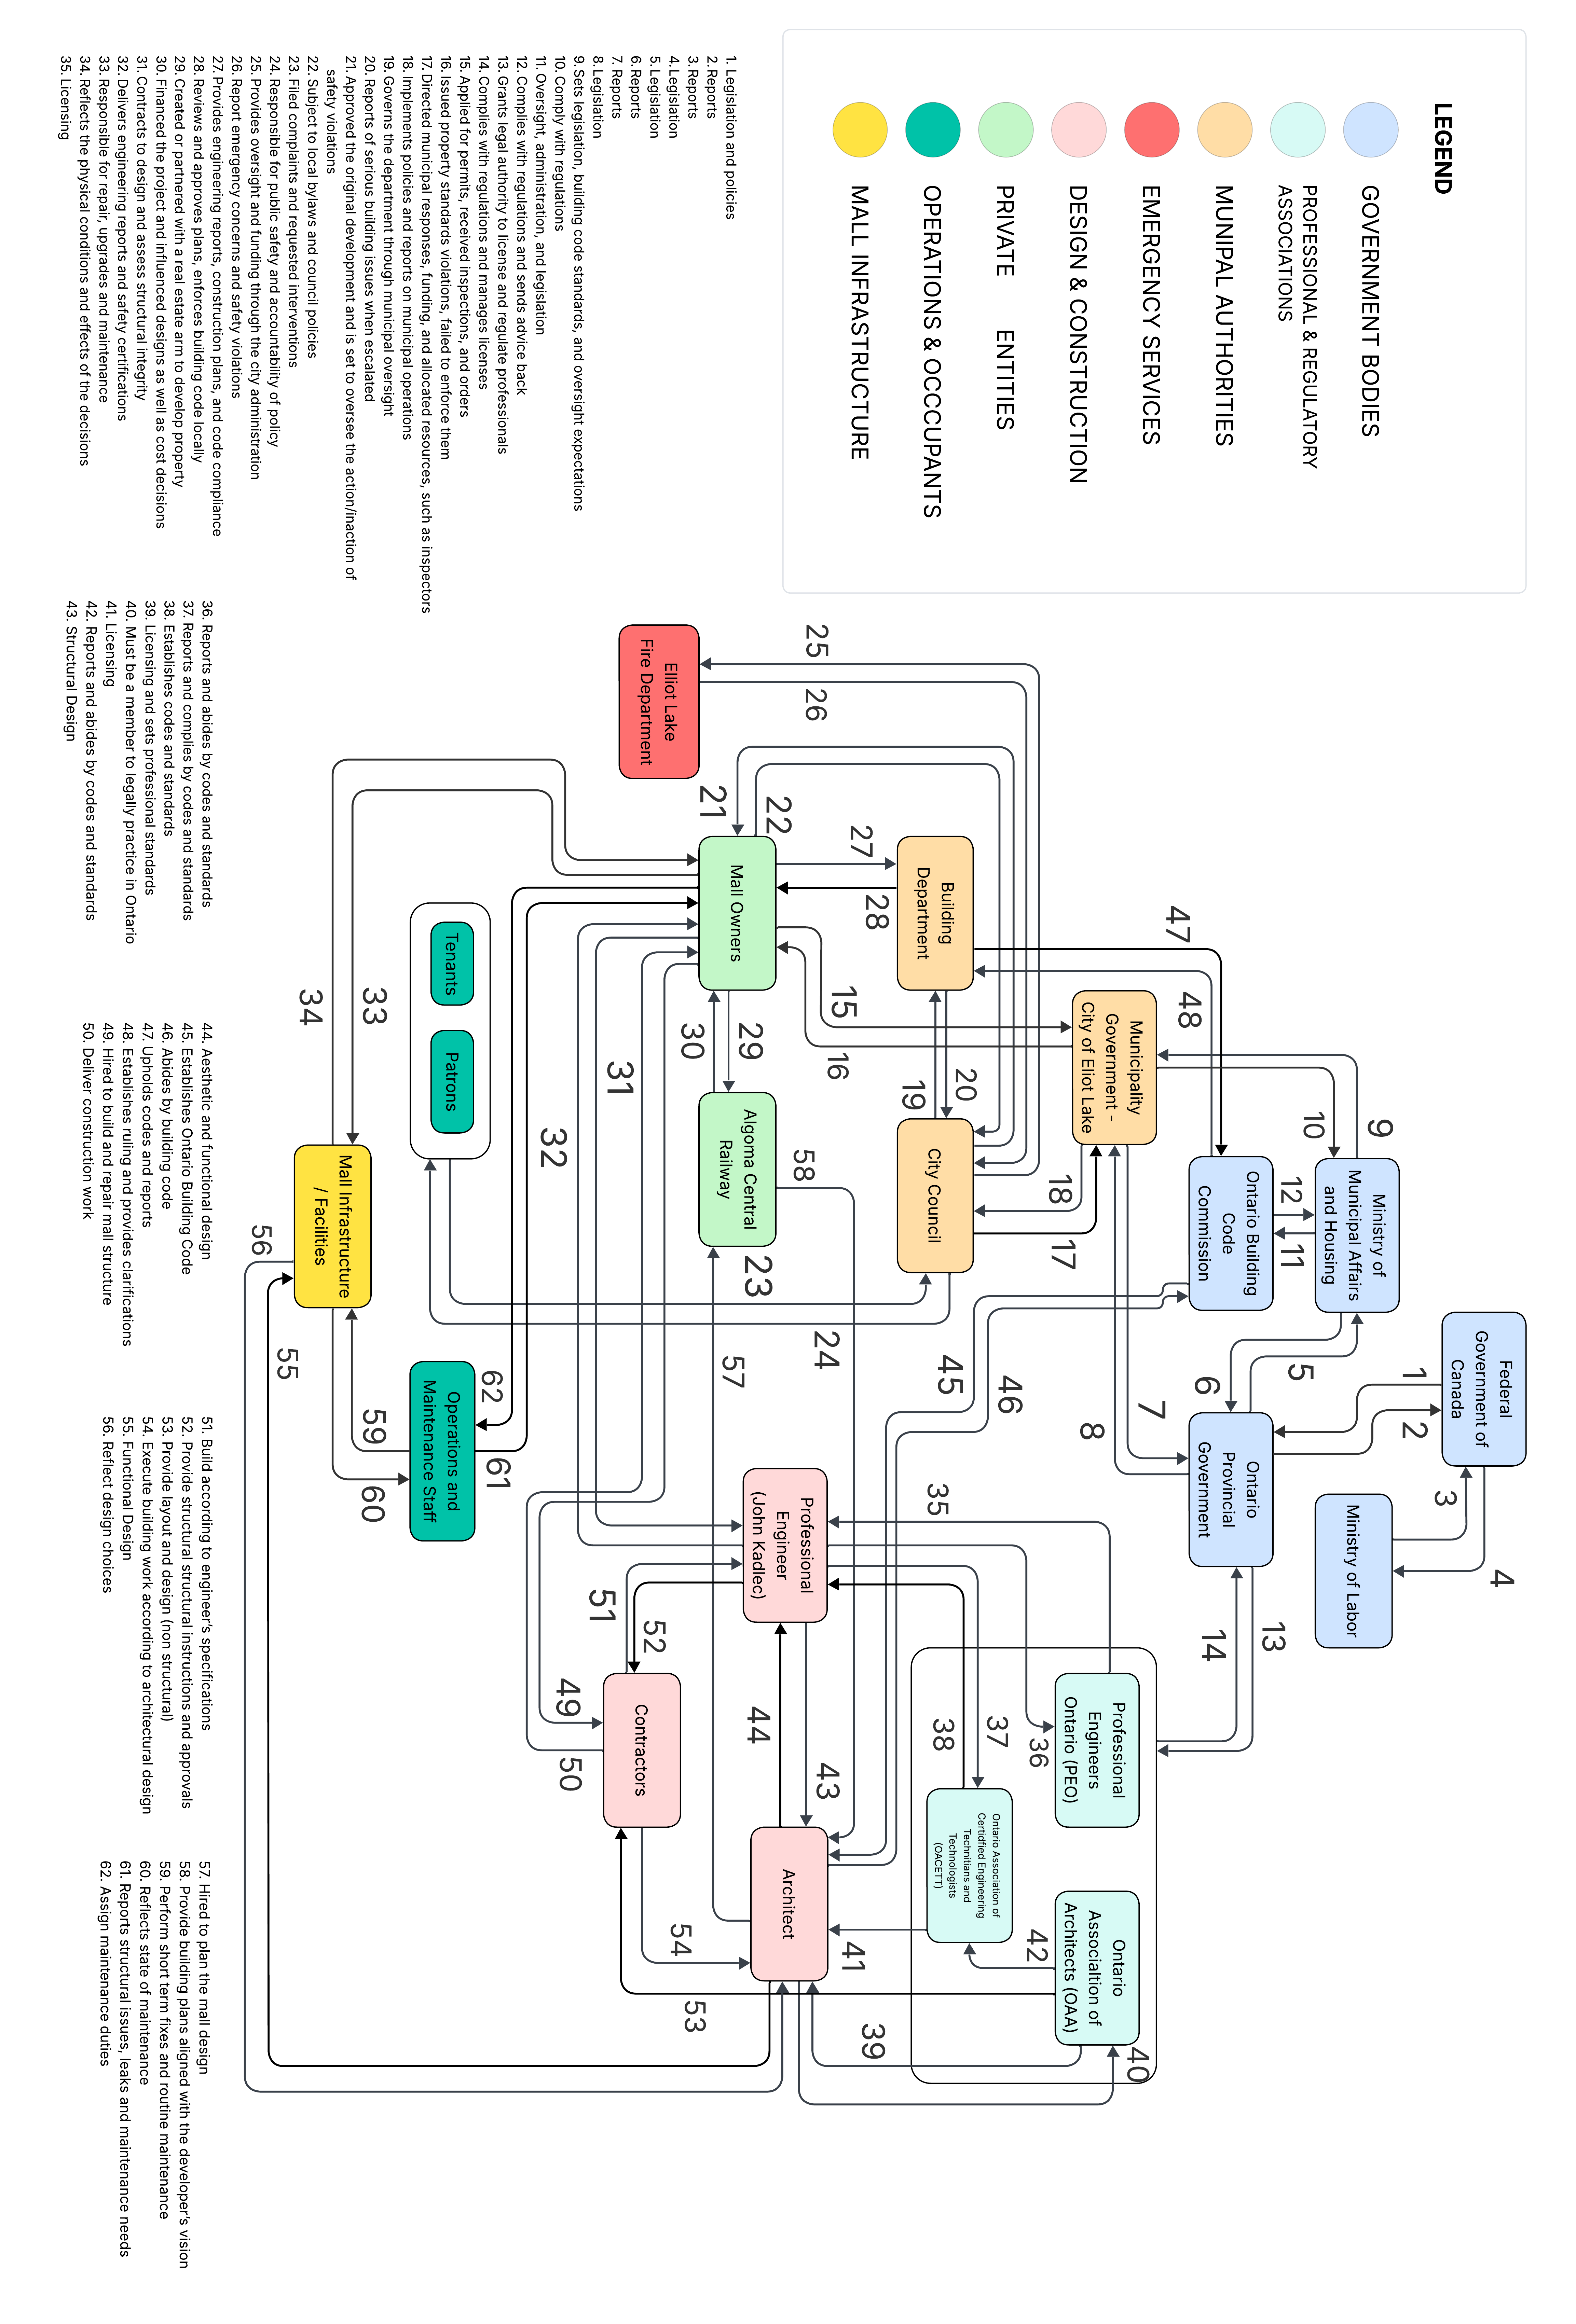
\includegraphics[height=0.8\paperheight]{SafetyControlStructure.png}
    \caption{Hierarchical Safety Control Structure of Algo Centre Mall}
    \label{fig:SCS}
\end{figure}

\begin{figure}[p]
    \centering
    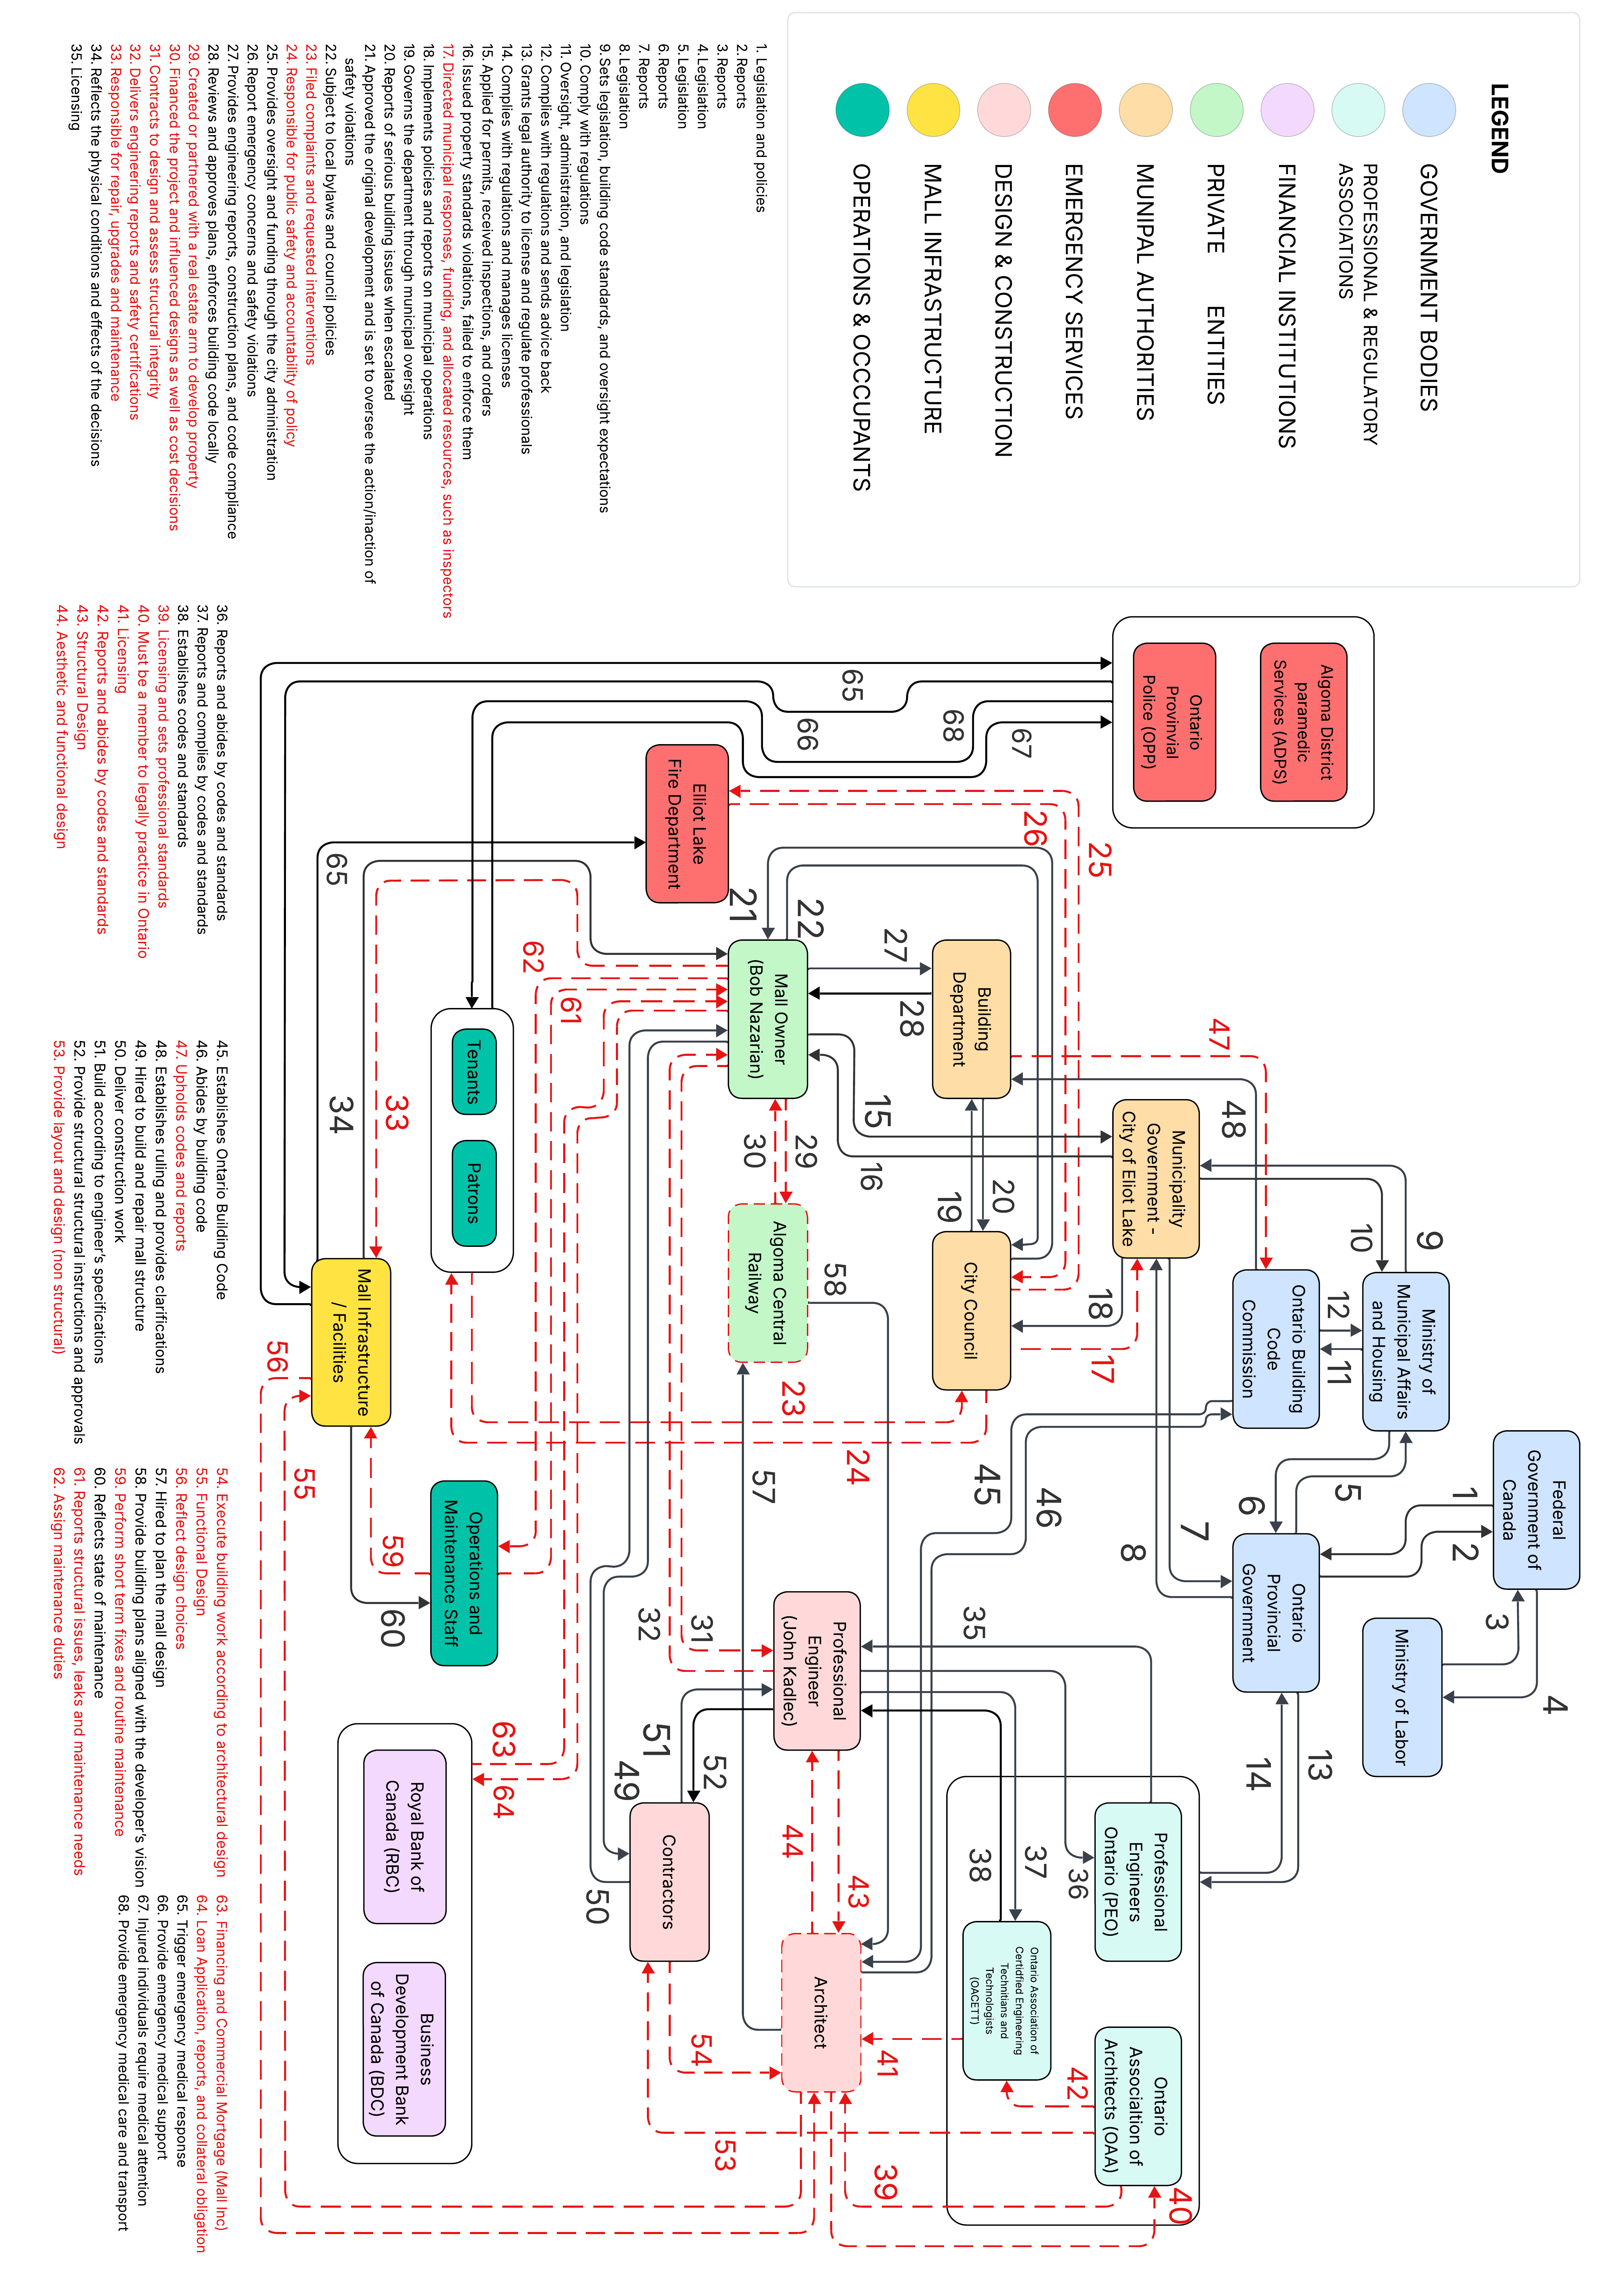
\includegraphics[height=0.78\paperheight]{SafetyControlStructure-Failure.png}
    \caption{Hierarchical Safety Control Structure of Algo Centre Mall at the time of the collapse. The control mechanisms that contributed to the collapse are highlighted in red.}
    \label{fig:SCS_broken}
\end{figure}

% \restoregeometry

\section{CAST Step 3: Bottom-up Analysis of the Safety Control Structure Components}
% Author: Wenxuan Meng
% Reviewer: Shuhan Zhneg

In this section, each component of the safety control structure of the Algo Mall is analyzed to see the role it played in its collapse.

\subsection{Federal Government of Canada}

The federal government's involvement in this case reveals how a broken governance system can allow serious safety issues to fall through the cracks. While federal agencies often occupy space in buildings like the Algo Mall, their occupancy does not guarantee responsibility to the building they occupy. This disconnect between public presence and regulatory accountability contributed to a situation where federal facilities gave the appearance of legitimacy and safety to a building that was, in fact, deeply unsafe. In addition, the slow mobilization of federal resources following the collapse undermined public trust and raised questions about the responsiveness of federal institutions to crises in smaller or more remote communities, such as Elliot Lake. The case of Algo Centre Mall highlights the need for more integrated oversight and better-defined roles for federal actors in ensuring the safety of the public facilities they use, regardless of ownership.

\subsubsection*{Safety Requirements and Responsibilities}

The federal government is expected to support public safety by enforcing and maintaining national legislation such as the Criminal Code, funding and overseeing federal agencies like Public Safety Canada, and setting national standards through model codes such as the National Building Code of Canada (NBC). While the enforcement of building safety rests with provincial and municipal authorities, the federal government influences safety practices by publishing national codes and funding research through institutions like the National Research Council. In the context of the Algo Centre Mall, the federal government also bears a duty to ensure that spaces leased by federal departments, such as Service Canada and Members of Parliament's offices, are reasonably safe for the public and for federal employees. Additionally, the federal government is responsible for providing coordinated emergency response support, particularly when provincial or municipal capabilities are overwhelmed.

\subsubsection*{Context in Which Decisions Were Made}

The federal government's actions must be understood in light of the legal boundaries of Canada's federal system. Construction safety is largely a provincial responsibility, and while the federal government produces the NBC, it lacks the constitutional authority to enforce its conditions or arrangements. The Algo Centre Mall, a privately owned and municipally regulated structure, was under the authority of the City of Elliot Lake and the Province of Ontario. Federal agencies that leased office space within the Mall had limited mechanisms, or perhaps little perceived obligation, to investigate or respond to ongoing deterioration in the building's structure. This resulted from a wider political context characterized by limited financial resources and federal intervention in local infrastructure matters during the early 2010s. When the collapse occurred, the federal government did not immediately intervene in rescue efforts. Only after significant public pressure and the direct involvement of Ontario Premier Dalton McGuinty did federal resources, such as a specialized crane from Toronto, become available to assist in search and rescue operations.

\subsubsection*{Mental Model}

Within the federal system, policymakers likely operated on the assumption that provincial and municipal authorities were managing the structural safety of the Algo Centre Mall. There appears to have been a widespread belief that once a building was approved and certified under local building codes, it did not require further intervention from federal tenants or agencies. This reflects a mental model in which liability and responsibility were seen to reside with the property owner and municipal inspectors, rather than with federal leaseholders. Additionally, it is likely that federal departments viewed their facilities management obligations in commercial leases narrowly, focusing on lease terms and tenant services rather than structural safety. There may also have been an implicit trust in the municipal permitting and inspection routine, which masked the serious long-term structural risks the Mall posed to federal employees and citizens alike.

\subsubsection*{Inadequate Control Actions}

The federal government failed to take a number of actions that could have mitigated the risk or severity of the disaster. Most notably, it did not institute any independent inspections of leased commercial properties despite the clear public-facing function of federal offices located in structurally deteriorating buildings. This constitutes a failure to provide a required safety control action. Furthermore, following the collapse, federal intervention in the emergency response was delayed and occurred only after significant provincial and public pressure. This represents a correct control action applied too late to affect the outcome. There is no evidence that the federal government attempted to proactively assess safety oversight mechanisms for leased properties even after the collapse, which suggests a lack of follow-through or revision of internal models for building safety. No unsafe or actively harmful actions were taken, but the federal government's inaction, especially in the face of known structural degradation, can be seen as a form of failure within the safety control structure.

\subsection{Ontario Provincial Government}

The role of the Ontario provincial government in this case reflects the dangers of distributed power without adequate accountability or support. By assigning municipalities the legal duty to enforce building safety while retaining little oversight of how those duties were performed, the province created conditions where gaps in enforcement could grow unchecked. In Elliot Lake, that dynamic allowed a structurally unsound building to remain in operation for decades despite widespread awareness of its problems. The province's failure to provide periodic structural inspections, combined with weak coordination in emergency response, exposed both regulatory and operational vulnerabilities.

Moreover, the case highlights how fragmented responsibilities and isolated ministries undermine systemic safety. Engineers, inspectors, labour officers, and emergency managers operated in parallel with insufficient mechanisms to synthesize their observations into collective action. Without structural changes to execute inspections, support local enforcement, and unify safety oversight, the same conditions that enabled the Algo Mall collapse could easily reemerge elsewhere in Ontario. The tragedy thus revealed the inadequacy of relying on self-correcting systems in contexts where power, expertise, and incentives are not aligned.

\subsubsection*{Safety Requirements and Responsibilities}

The Ontario provincial government holds primary responsibility for regulating and enforcing building safety within the province. Through legislation such as the Building Code Act and the accompanying Ontario Building Code, the province sets minimum design and construction standards for all buildings under its power. It also has oversight of professions such as engineers and building officials through special authorities like Professional Engineers Ontario (PEO) and the Ontario Building Officials Association (OBOA). The Ministry of Municipal Affairs and Housing is tasked with maintaining and updating the Building Code, while the Ministry of Labour, Immigration, Training and Skills Development (formerly the Ministry of Labour) ensures workplace safety and may intervene in matters involving hazardous conditions. Additionally, the province is responsible for empowering municipalities to enforce building codes and property standards, and is expected to ensure that those local governments have the capacity and guidance needed to fulfill those obligations.

In the case of emergency response, Ontario's Ministry of the Solicitor General and its Emergency Management Ontario branch have the power for oversight and coordination of provincial-level emergency preparedness. In contexts like the Algo Mall collapse, the province is expected to provide expertise, specialized equipment, and decision-making support in rescue operations that exceed municipal capabilities. Furthermore, the province is responsible for establishing clear lines of authority and communication between engineering professionals, municipalities, and provincial ministries during both routine safety enforcement and crisis events.

\subsubsection*{Context in Which Decisions Were Made}

The Ontario provincial government's actions must be understood in the context of a system that transfers primary responsibility for enforcing the Building Code to municipalities, while retaining authority over the standards themselves. Since the 1990s, there had been a political trend toward ``downloading'' responsibilities onto municipalities in Ontario, particularly under governments that have limited resources. This left smaller municipalities like Elliot Lake under-resourced, even as they remained legally accountable for enforcing complex safety standards. At the same time, the province retained the authority to intervene in matters of non-compliance with the Code, particularly when municipalities failed to act. However, this authority was not exercised in the case of Algo Mall.

Additionally, at the time of the collapse in 2012, there was no mandatory requirement in Ontario for periodic inspections of structural elements in existing buildings. Provincial oversight of engineering practice existed but relied heavily on self-regulation by PEO. The Ministry of Labour, though notified at times of hazardous working conditions at the Mall, did not act on the escalating structural risk as a workplace safety issue. In terms of emergency response, the province did not immediately provide direct support after the collapse. When municipal rescuers declared the structure too unsafe to enter, the absence of a provincial-level command mechanism left the situation paralyzed for over 48 hours, until political intervention from the Premier's Office jump-started further rescue efforts.

\subsubsection*{Mental Model}
The provincial government appeared to operate under the assumption that municipalities were adequately equipped and motivated to enforce structural safety standards on their own. This mental model underestimated the capacity gaps in smaller municipalities and failed to account for the complex political and economic incentives facing local officials, such as avoiding enforcement actions that could destabilize a community's economic hub. Additionally, the province seemed to assume that periodic structural inspection of buildings was unnecessary unless complaints or renovations were involved, despite the known aging infrastructure across many Ontario communities.

In the context of the Algo Mall, provincial ministries may have lacked the internal information-sharing structures necessary to connect separated indicators of risk. For example, the Ministry of Labour was aware of ongoing leaks and employee safety concerns within the Mall but did not interpret these as a symptom of structural decay requiring higher-level intervention. Similarly, the Ministry of Municipal Affairs and Housing had no formal mechanisms to monitor municipal enforcement of the Building Code. The overall process model implicitly placed trust in local authorities while offering limited oversight or support, an arrangement that ultimately failed when multiple warning signs went ignored over many years.

\subsubsection*{Inadequate Control Actions}
The province failed to take several critical control actions that could have prevented or mitigated the collapse. Most significantly, it did not require ongoing structural inspections for aging commercial properties, even though other jurisdictions (such as Quebec) had begun implementing such practices following earlier tragedies \cite[p.585-586]{AlgoLakeReport1}. The provincial government also failed to monitor or assess the enforcement capacity of small municipalities like Elliot Lake, which struggled with both technical knowledge and political pressures in dealing with problem buildings. Furthermore, despite being notified of concerns about the Mall over the years, through both Ministry of Labour interactions and public reports, the province took no steps to independently investigate or intervene in enforcement lapses.

Following the collapse, the province's initial failure to take command of the rescue operation led to a dangerous delay in life-saving action. The decision to suspend rescue efforts due to structural instability was reasonable in itself, but the lack of an alternative plan, as well as an apparent vacuum of leadership, represented a breakdown in emergency management coordination. It was only after Premier Dalton McGuinty intervened personally that the necessary equipment and expertise were brought in to resume search efforts. This reveals a significant misalignment between the province's formal responsibilities and its operational readiness to act in a crisis.

\subsection{Municipal Government - City of Elliot Lake}

The failures of the municipal government illustrate how small-town politics, economic dependency, and institutional isolation can undermine safety enforcement. Elliot Lake's officials were embedded in a system that discouraged confrontation with powerful local stakeholders, especially the owners of economically important infrastructure. The City's reluctance to enforce safety regulations stemmed not only from limited resources but from a broader civic culture that emphasized stability over accountability \cite[p6-7, p380-386]{AlgoLakeReport1} (Elliot Lake Commission of Inquiry, 2014, pp. 6-7, 380-386).

This case reveals the fragility of relying on municipal enforcement in contexts where political and economic incentives are misaligned with public safety. Without strong oversight from the provincial level and without a robust culture of documentation, transparency, and accountability, small municipalities can become structurally incapable of acting on known risks. The City of Elliot Lake's failures were not just procedural; they were cultural and systemic. The Commission concluded that these failures contributed directly to the deaths of Lucie Aylwin and Doloris Perizzolo, and that a stronger municipal leadership could have prevented the tragedy.

\subsubsection*{Safety Requirements and Responsibilities}

As an authority under Ontario's Building Code Act, the City of Elliot Lake had the legal responsibility to enforce the Ontario Building Code (OBC) within its jurisdiction. This included issuing building permits, inspecting construction and renovations, and taking enforcement action against buildings that failed to comply with minimum standards. In addition to its responsibilities under the OBC, the municipality was also obligated to enforce local property standards bylaws, such as those governing maintenance, structural soundness, and occupancy safety, through its municipal Property Standards Officer and Chief Building Official (CBO) \cite[p380-381]{AlgoLakeReport1}.

As the owner of public infrastructure and a regulator of private buildings, the City held a dual role: one as a watchdog of community well-being and another as an enforcer of provincial safety laws. This placed the City in a position of both legal responsibility and moral authority to act decisively when confronted with evidence of deteriorating structures like the Algo Centre Mall.

\subsubsection*{Context in Which Decisions Were Made}

The actions of the City of Elliot Lake were shaped by its constrained political, economic, and administrative environment. Following the closure of uranium mines in the 1990s, the City had gone through a long-term economic decline, becoming heavily reliant on retirement tourism and the commercial activity generated by the Mall. By 2012, the Algo Centre was a symbolic and economic hub of the city. This context contributed to a pervasive reluctance to take enforcement actions that might result in the Mall's closure or economic destabilization \cite[p6-7, p380-381]{AlgoLakeReport1}.

These pressures resulted from a lack of administrative capacity and technical independence. The City relied heavily on its contracted Chief Building Official, who often worked in isolation and had limited support or oversight. The Commission found that municipal officials were aware of long-standing water leakage and public complaints, yet consistently deferred to property owners or private engineers, choosing not to issue work orders or pursue more direct enforcement strategies. Decisions were frequently based on informal conversations and unwritten understandings, rather than documented inspections or formal code enforcement proceedings \cite[p378-380]{AlgoLakeReport1}.

\subsubsection*{Mental Model}

The City of Elliot Lake operated with a deeply constrained process model, in which the primary goal was to maintain economic stability and civic calm. This model privileged compromise and continuity over risk detection or enforcement. Municipal staff, particularly the CBO and Property Standards Officer, repeatedly relied on verbal assurances from building owners or engineers, rather than objective evidence or detailed inspections. As the Inquiry report notes, ``there was an almost unshakable belief in the integrity of the building and in the private engineers hired by the owner''.

Moreover, municipal officials appeared to adopt a minimalistic interpretation of their enforcement powers. They believed that unless a structure was obviously unsafe or unless an engineer explicitly declared it dangerous, the City had little authority or obligation to act. This perspective ignored the broader purpose of the OBC and property standards regulations, to prevent precisely the kind of systemic decay that affected the Mall. The process model in place did not allow for anticipation, escalation, or intervention, even in the face of decades-long evidence of deterioration.

\subsubsection*{Inadequate Control Actions}

The City of Elliot Lake failed to take multiple control actions that were within its power and duty. Most significantly, it did not issue any work orders or property standards orders that would have required the Mall's owners to repair persistent water infiltration or corrosion of the structural steel. Nor did it demand independent structural assessments once it became clear that the original waterproofing had failed and the Mall was suffering from ongoing leaks and ceiling collapses \cite[p380-385]{AlgoLakeReport1}. Even after the 2008 resignation of an engineer hired by the owner, who cited professional concerns about the structural safety of the roof-deck parking system, the City did not act on the warning or require further investigation.

The City also failed to keep adequate records of complaints, inspections, or enforcement decisions. As a result, institutional memory was limited, and repeated red flags did not accumulate into a pattern that might have triggered more serious intervention. The lack of documentation made it easy for officials to deny prior knowledge or to frame each concern as an isolated incident, rather than part of a larger trend of systemic neglect.

Finally, during the emergency response, the City was slow to coordinate with provincial agencies and did not have a prepared plan for managing structural collapse or requesting heavy urban rescue equipment. This further delayed life-saving interventions in the critical hours after the collapse.

\subsection{Professional and Regulatory Associations}
The Algo Centre Mall collapse exposed systemic weaknesses across multiple professional and regulatory associations. These bodies, tasked with upholding professional standards, licensing qualified practitioners, and protecting the public interest, demonstrated a shared failure to anticipate, detect, or respond to declining safety in a high-risk structure. Their inaction reveals a broader issue: self-regulation, without proactive monitoring or accountability mechanisms, can foster conditions in which negligence goes unchecked.

Though their mandates differ, associations such as Professional Engineers Ontario (PEO), the Ontario Association of Architects (OAA), and the Ontario Association of Certified Engineering Technicians and Technologists (OACETT) all played passive roles in the years leading up to the collapse. Despite warning signs, disciplinary histories, and controversial engineering assessments, none of these organizations took preemptive action to safeguard the public. Their governance models relied heavily on formal complaints, assumed professional integrity, and lacked mechanisms to identify practitioners operating at the edge of competence or ethics. The tragedy underscores the need for professional bodies to evolve beyond gatekeeping and disciplinary functions into active safety participants \cite[p393–396]{AlgoLakeReport1}.

\subsubsection*{Safety Requirements and Responsibilities}

Professional regulatory associations are responsible for licensing and regulating their members in accordance with public safety mandates. PEO oversees professional engineers, OAA governs licensed architects, and OACETT certifies technologists and technicians. Each organization is tasked with setting entry standards, enforcing codes of conduct, and taking disciplinary action when members pose risks to public welfare. In the context of the Algo Mall, these bodies were expected to monitor practitioner competence, investigate potential misconduct, and issue guidance or intervention where safety risks emerged \cite[p393]{AlgoLakeReport1}.

They also hold a duty to support the ethical practice of members working in high-risk contexts, offering standards of care, alerts, or training related to infrastructure aging, engineering ethics, and the escalation of risk \cite[p396]{AlgoLakeReport1}.

\subsubsection*{Context in Which Decisions Were Made}

At the time of the collapse, all three associations operated under complaint-driven disciplinary models. Their investigations were triggered only after formal complaints were filed, often long after questionable decisions had already produced harm. Even in cases where members had been previously disciplined, such as Robert Wood, no proactive monitoring or oversight mechanisms were in place to track future risk \cite[p394]{AlgoLakeReport1}. This hands-off approach allowed dangerous practices to persist undetected, particularly in smaller communities where institutional checks were weak or absent.

Furthermore, these associations functioned in isolation from one another. There were no cross-professional accountability structures to review safety threats involving multi-disciplinary coordination, such as joint engineering and architectural failures. No coordinated guidance was offered in relation to high-risk properties or aging infrastructure, despite the Mall’s ongoing deterioration being widely known in Elliot Lake (pp. 393–394).

\subsubsection*{Mental Model}

The mental model underlying these associations appeared to rest on assumptions of professional self-governance and reactive enforcement. They presumed that licensed professionals would act ethically and that serious misconduct would be brought forward by clients, colleagues, or the public. This placed regulatory action downstream of visible failure, rather than positioning associations as upstream actors in systemic safety oversight \cite[p394–395]{AlgoLakeReport1}.

There was also a heavy reliance on legal formalism: associations appeared more focused on protecting procedural fairness for members than on creating accessible, timely, or proactive mechanisms for public protection. Their models did not incorporate strategies for risk-based review, early intervention in high-risk cases, or the monitoring of repeated concerns across multiple files \cite[p396]{AlgoLakeReport1}.

\subsubsection*{Inadequate Control Actions}

None of the associations investigated the involved engineers or issued disciplinary warnings prior to the collapse, despite multiple red flags. PEO failed to act on Robert Wood’s continued work following earlier discipline and did not review his 2012 inspection report, which contradicted clear structural indicators \cite[p393–394]{AlgoLakeReport1}. The OAA did not issue any guidance or initiate a review of architectural contributions to the Mall’s failure. OACETT did not clarify the boundary of accountability for technologists involved in design and inspection support roles \cite[p396]{AlgoLakeReport1}.

Following the collapse, PEO initiated an investigation into Wood, but this came only after fatalities had occurred. The other associations did not appear to respond in any meaningful systemic way. No association used the tragedy to immediately reform complaint procedures, implement proactive member reviews, or strengthen risk oversight for aging infrastructure contexts \cite[p396]{AlgoLakeReport1}.

\subsection{Mall Owners}

The role of the Mall owners in this disaster illustrates how private interests, when unchecked by effective oversight, can become active contributors to public risk. While property owners are assumed to act as managers of their buildings, this case demonstrates how economic pressures, regulatory gaps, and weak enforcement systems can encourage neglect and even deception. Nazarian's actions were shaped not only by financial self-interest but by the absence of meaningful consequences. Municipal inspectors failed to hold him accountable, and professional engineers continued to work with him even after safety concerns were ignored.

This case exposes a dangerous imbalance in Ontario's building safety structure: the assumption that private owners will act rationally in the public interest is not valid in high-risk, low-capacity environments. The Mall's deterioration was not sudden. It was persistent, visible, and preventable. Yet the institutional structure allowed an owner with clear conflicts of interest to override professional advice and suppress risk information. As the Commissioner concluded, the collapse of the Algo Centre Mall was not a random tragedy but the predictable result of years of regulatory and ethical failure, with the owner playing a central role \cite[p6-7, p243-248]{AlgoLakeReport1}.

\subsubsection*{Safety Requirements and Responsibilities}

As private property owners and landlords, the owners of the Algo Centre Mall were legally responsible for ensuring that their building met structural safety standards and that it was maintained in a condition that did not pose a hazard to occupants or the public. This included complying with municipal property standards bylaws and ensuring that necessary repairs were performed in accordance with the Ontario Building Code. The owners were also expected to act upon advice from professional engineers and to commission timely inspections and repairs when structural issues were suspected or identified. Their responsibilities extended beyond tenant comfort to include a duty of care to the public and legal accountability under civil and potentially criminal law for failures that result in harm \cite[p160-161, p171-172]{AlgoLakeReport1}.

From the time of the Mall's construction in 1979 until its collapse in 2012, the building passed through several different owners. While the identity of the legal owner changed, each successive owner inherited the same responsibilities to manage, repair, and maintain the structure, especially its compromised waterproofing system and deteriorating steel supports.

\subsubsection*{Context in Which Decisions Were Made}

Throughout the Mall's history, particularly from the 1990s onward, the owners operated under a persisting state of financial constraint and deferred maintenance. The building suffered from a known design flaw: the rooftop parking deck allowed water to leak directly onto the structural steel below, initiating corrosion that worsened over decades. Rather than investing in a complete repair or membrane replacement, successive owners, including Eastwood Mall Inc. under Bob Nazarian, chose temporary patchwork solutions such as sealing membranes or partial grouting \cite[p183-185, 243-245]{AlgoLakeReport1}.

By the late 2000s, the corrosion had become extensive and visible. In 2009, Nazarian sought to refinance the Mall through a loan from Royal Bank of Canada and later a mortgage insurer. During this process, he withheld engineering reports and failed to disclose the full extent of the building's deterioration. His conduct during these years was shaped by financial desperation and a clear attempt to avoid major capital expenditures. The Inquiry found that Nazarian knowingly prioritized financial survival over public safety, concealing reports and ignoring engineers' recommendations for serious structural repairs \cite[p346-248]{AlgoLakeReport1}.

\subsubsection*{Mental Model}

The Mall owners, especially during the final years of the Mall's life, appeared to operate with a self-serving and dangerously flawed mental model. They viewed the Mall primarily as a financial asset, to be maintained only to the extent necessary to preserve cash flow and avoid tenant losses. Structural deterioration was treated as a cost management issue rather than a life safety concern. When engineering reports raised concerns, Nazarian routinely downplayed their severity or rejected them. In one case, he failed to submit an engineer's report to a mortgage insurer because it could harm refinancing \cite[p246-247]{AlgoLakeReport1}.

Rather than viewing engineers as trusted safety professionals, the owner treated them as service providers whose recommendations could be accepted or rejected based on cost. This stance toward engineering advice created a culture of non-compliance, in which the most urgent warnings were ignored, and consultants were pressured to revise their language or conclusions. Nazarian's mental model did not prioritize systemic risk or duty of care. It prioritized short-term monetary feedback and public appearance.

\subsubsection*{Inadequate Control Actions}

The Mall owners failed to take virtually every control action necessary to prevent structural failure. They ignored or minimized multiple engineering assessments warning of serious corrosion and structural risk. For instance, a 2009 report explicitly described rust, metal loss, and the risk of collapse if deterioration continued unchecked. Yet no meaningful repairs were carried out \cite[p245-246]{AlgoLakeReport1}. The owner repeatedly delayed or cancelled planned repairs, citing costs or concerns about tenant disruptions.

In some cases, the owner set out to actively mislead stakeholders. During refinancing negotiations, Nazarian failed to disclose engineering reports that would have revealed the Mall's compromised condition. When engineers offered assessments that were too critical, he sought more vague opinions from others. The result was a pattern of behavior in which risks were deliberately concealed or reframed to avoid triggering costly interventions. These actions were not just inadequate; they were recklessly unconcerned about public safety and regulatory obligations.

\subsection{Building Department – Robert Wood}

Robert Wood's dual roles, as former CBO and then retained engineer, highlight the ethical and structural vulnerabilities that can emerge in small municipalities where regulatory and professional roles blur. His case illustrates how individual professional failures can become systemic when oversight is weak, institutions are deferential, and warning signs are normalized. Wood was not someone operating outside of institutional norms; rather, his behaviour reflected a broader culture of accommodation, risk tolerance, and procedural minimalism.

The Commission criticized Wood for prioritizing his professional relationship with the client over his duty to the public. It emphasized that engineers must not only act competently but must resist pressure to provide convenient or optimistic assessments when evidence suggests otherwise \cite[393-396]{AlgoLakeReport1}. The tragedy underscores the need for stronger systems of peer review, public disclosure, and escalation protocols when engineers are working in high-risk, publicly occupied buildings.

\subsubsection*{Safety Requirements and Responsibilities}

Robert Wood played a dual role in the Algo Centre Mall disaster. First, as a professional engineer contracted by the Mall's owner, he was responsible for conducting structural assessments and providing expert evaluations of the integrity of the Mall's structure. Second, prior to that role, he served as Chief Building Official (CBO) for the City of Elliot Lake, where he was tasked with enforcing the Ontario Building Code and ensuring that buildings under his jurisdiction complied with safety regulations. As both an engineer and a former municipal official, Wood held professional and ethical obligations to protect public safety, provide objective assessments, and disclose critical structural deficiencies \cite[p374-377, p387-388, p393-396]{AlgoLakeReport1}.

As an engineer licensed by Professional Engineers Ontario (PEO), Wood was expected to act with independence, competence, and integrity. His reports and judgments carried significant weight with building owners, tenants, financial institutions, and municipal authorities.

\subsubsection*{Context in Which Decisions Were Made}

In 2009, Wood left his role as CBO and began working privately. He was later recruited by Bob Nazarian to inspect the Mall in 2012, just weeks before its collapse. In this capacity, Wood conducted a visual inspection of the rooftop parking deck and issued a report stating that the structure was safe and that no immediate repairs were necessary. This report played a key role in reassuring the owner, tenants, and the public that the Mall remained safe to occupy \cite[p392-394]{AlgoLakeReport1}.

However, his inspection was extremely limited: Wood failed to review prior engineering reports, did not perform intrusive testing, and did not fully investigate visible corrosion or water damage. Despite having access to documentation describing years of water infiltration, prior resignations by other engineers, and visual evidence of structural decay, Wood minimized the risks and declared the building fit for continued occupancy. The Commission concluded that his assessment was not only incorrect but largely negligent given the context \cite[p393-394]{AlgoLakeReport1}.

\subsubsection*{Mental Model}

Wood appeared to operate under a dangerously flawed mental model that prioritized client satisfaction over public safety. He relied heavily on visual cues and interpreted his role narrowly, treating the inspection as a surface-level task rather than a serious investigation of known structural issues. Despite knowing that he was evaluating a building with a history of leaks and visible corrosion, he failed to recognize, or chose to ignore, the systemic risks posed by the failing rooftop parking structure.

His mental model also seemed shaped by familiarity and confidence. Having previously worked as the CBO in Elliot Lake, he may have developed an overly informal relationship with the built environment and its political stakeholders. Rather than adopting a precautionary or skeptical approach, Wood accepted the owner's framing of the issues and interpreted them as cosmetic or low-risk. This lack of professional distance significantly compromised his judgment.

\subsubsection*{Inadequate Control Actions}

Robert Wood's conduct represents one of the most critical failures in the safety control structure. His engineering report, completed in May 2012, concluded that the building remained structurally sound, a conclusion that directly contradicted years of warning signs and photographic evidence of severe corrosion. This assessment gave the Mall's owner justification to defer repairs and to continue operating the facility. The Commission found that Wood's report was materially deficient and failed to meet the standard of care expected of a professional engineer \cite[p393-394]{AlgoLakeReport1}.

Moreover, Wood did not recommend follow-up evaluations, additional testing, or structural reinforcement, despite observing signs that the rooftop beams had suffered significant damage. He also failed to alert municipal officials or regulatory authorities, even though he had reason to believe the building was not safe. His actions constituted both a failure to provide required control actions and a provision of incorrect, unsafe information that contributed directly to the conditions of collapse.

Following the collapse, PEO initiated disciplinary proceedings against Wood. The fact that such action only occurred after fatalities underscores the inadequacy of both Wood's own decisions and the broader system of accountability within which he operated.

\subsection{Tenants – Occupants of the Algo Centre Mall}
The experience of the tenants in the Algo Centre Mall illustrates how those closest to danger can become desensitized to it, particularly in environments of economic fragility and institutional trust. Tenants did observe warning signs, but lacked the power, resources, or organizational capacity to take decisive action. Their continued presence lent legitimacy to the Mall and masked its dangers, but broader structural forces constrained their options: a weak local economy, lack of alternative space, and a fragmented system of safety governance.

This case also demonstrates how the assumption that tenants or the public will raise an alarm when something is wrong can be dangerously misplaced. In complex systems, the silence of those at risk is not always a sign of safety. It may be a symptom of normalization. The Commission acknowledged this complexity, noting that tenants were in many ways victims of the same systemic neglect that ultimately led to the collapse \cite[p250–251]{AlgoLakeReport1}.

\subsubsection*{Safety Requirements and Responsibilities}

The tenants of the Algo Centre Mall, including retailers, service providers, government offices, and financial institutions, were responsible for ensuring the safety of their leased spaces for staff and customers, within the limits of their control. While they were not building owners and did not hold regulatory authority, tenants are expected to report safety hazards to landlords and municipal officials and may also be expected to take independent action if a space appears dangerous to occupy. Their feedback, complaints, or withdrawal of business can exert pressure on property owners to address maintenance issues. Tenants also help shape public perceptions of safety through their continued presence or absence in a facility.

Among the most prominent tenants were the Royal Bank of Canada, Service Canada, the Ontario Ministry of Health, a food court, and various retail businesses. These tenants provided services central to the daily life of Elliot Lake residents, many of whom were retired and relied on the Mall as both a commercial and social hub \cite[p249–251]{AlgoLakeReport1}.

\subsubsection*{Context in Which Decisions Were Made}

Over the years, tenants became increasingly aware of the physical deterioration of the Mall. Leaks were persistent and widely reported; ceiling tiles stained or collapsed due to water damage; rust and corrosion were visible in some areas. Tenants routinely complained to the Mall management, and some attempted to pressure the landlord to make repairs. However, despite years of reporting these issues, repairs were minimal or cosmetic, and the building continued to degrade. Tenants had limited legal leverage and were economically vulnerable: for many small businesses, relocating to another facility was not feasible, and the Mall remained the only possible commercial centre in the city \cite[p244–251]{AlgoLakeReport1}.

Some larger tenants, such as the Royal Bank of Canada, did begin making exit plans. RBC formally notified the landlord in 2011 that it would not renew its lease beyond 2013, citing concerns about the building's condition. Still, the Bank continued to operate in the Mall until the collapse in 2012. Many smaller tenants lacked such flexibility. Others normalized the deterioration, treating it as a frustrating but routine part of operating in Elliot Lake.

\subsubsection*{Mental Model}

Most tenants appeared to operate with a resigned, incremental view of the risks. Their mental model framed the leaks, rust, and ceiling collapses as maintenance problems or aesthetic stains, not as signs of imminent structural failure. Even as conditions worsened, the absence of clear and direct warnings from engineers or building officials likely reinforced a belief that the building remained fundamentally safe. Tenants trusted that someone, whether the landlord, city inspectors, or engineers, was ultimately ensuring that the building remained within acceptable safety limits.

This mental model also reflected the community’s economic dependence on the Mall. Closing a business or demanding relocation could mean the loss of livelihoods or severing customer ties in a town with few alternatives. Tenants made calculated decisions to continue operations while hoping for improvements, assuming that structural failure was unlikely or that authorities would intervene if danger became real.

\subsubsection*{Inadequate Control Actions}

While the tenants had no formal role in building inspections or enforcement, some did fail to take stronger actions that might have mitigated risk. For instance, they could have issued public complaints, escalated concerns to provincial regulators, or collectively demanded third-party inspections. While some individual tenants did make complaints, there was no unified tenant effort to push for a structural review or to involve the media in highlighting the Mall’s deteriorating condition. Looking back, the normalization of risk and the dispersed, informal nature of tenant communications allowed dangerous conditions to persist without broader alarm \cite[p250–251]{AlgoLakeReport1}.

That said, many tenants operated under serious constraints. Small business owners feared losing their livelihoods; others were simply unaware of the full extent of the structural risk. The Inquiry recognized that tenants lacked the technical knowledge and authority to fully assess the situation and should not be seen as primarily responsible for the collapse.

\subsection{Emergency Services – Elliot Lake Fire, Police, EMS, and Urban Search and Rescue (USAR)}
The emergency response to the Algo Centre Mall collapse reveals the structural fragility of Ontario’s emergency preparedness for low-frequency, high-impact urban disasters, especially in remote communities. Local responders were heroic but under-equipped. Provincial coordination was slowed by unclear jurisdiction, policy rigidity, and an absence of integrated response protocols for structural collapse scenarios. This case highlights the importance of decentralizing emergency response capacity while maintaining strong intergovernmental coordination mechanisms.

More broadly, the collapse exposed a systemic bias toward routine over planning in emergency services. Municipalities and provincial agencies had planned for floods, fires, and severe weather, but not for structural collapse in a critical piece of infrastructure. The lack of real-time adaptability, specialized equipment, and rehearsed interagency protocols resulted in tragic consequences.

The Commission concluded that the failure was not rooted in individual incompetence but in a system unprepared for the extraordinary. In response, it recommended major reforms in training, resource deployment, USAR accessibility, and the formal integration of emergency services across jurisdictional boundaries \cite[p288–290]{AlgoLakeReport1}.

\subsubsection*{Safety Requirements and Responsibilities}

Emergency services, including the Elliot Lake Fire Department, local and provincial police, Emergency Medical Services (EMS), and, eventually, specialized Urban Search and Rescue (USAR) teams, held the legal and ethical responsibility to respond promptly and effectively to the Mall collapse. Their duties included scene assessment, categorization, search and rescue, and the coordination of emergency response efforts in accordance with Ontario’s emergency management legislation. The Municipal Emergency Control Group (MECG), which includes key emergency services and municipal leaders, was also responsible for activating the municipal emergency plan and requesting external support when the scope of a disaster exceeded local capabilities \cite[p282–284, 306–310]{AlgoLakeReport1}.

In particular, emergency services were tasked with balancing responder safety and the potential for life-saving action, coordinating with provincial officials, and communicating with the public in a transparent, timely manner.

\subsubsection*{Context in Which Decisions Were Made}

On June 23, 2012, the rooftop parking deck of the Algo Centre Mall partially collapsed into the building’s interior, trapping two people under the rubble. Local emergency services were immediately dispatched to the scene. Upon arrival, the scene was chaotic but not without precedence for the fire department and EMS. However, as responders began to assess the structural conditions, it became clear that the site posed serious secondary collapse risks. The Elliot Lake Fire Department, with limited personnel, equipment, and training in structural collapse scenarios, struggled to develop a safe and effective rescue strategy \cite[p282–286]{AlgoLakeReport1}.

Within hours, local responders requested provincial assistance. However, the system of escalation and resource mobilization was slow and poorly coordinated. The heavy urban search and rescue team (CAN-TF3), based in Toronto, did not arrive until June 25—more than 50 hours after the initial collapse. Compounding this delay was a breakdown in communication between the province and the municipal Emergency Operations Centre. A temporary halt to rescue operations due to safety concerns prompted public outcry and, eventually, a direct intervention by the Premier’s Office \cite[p284–288]{AlgoLakeReport1}.

\subsubsection*{Mental Model}

The mental model guiding local emergency services was constrained by limited training, jurisdictional ambiguity, and a procedural commitment to responder safety. Local responders acted with courage and urgency, but their process model lacked the depth required for rare, high-risk, low-frequency events like structural collapse. Their approach reflected a command-and-control mindset focused on perimeter safety and assessment, rather than adaptive coordination and improvisation under uncertainty.

Moreover, the process model at the provincial level, particularly for coordinating USAR deployment, was reactive, isolated, and bureaucratically sluggish. Provincial officials and CAN-TF3 had no preexisting agreements with municipalities for structural collapse support, nor clear guidelines for rapidly mobilizing resources outside the Greater Toronto Area. The result was a disconnected response where local services were overwhelmed, provincial support was delayed, and federal assets were not considered until after political intervention \cite[p284–289]{AlgoLakeReport1}.

\subsubsection*{Inadequate Control Actions}

The most consequential inadequate control action was the failure to sustain rescue operations during the critical early hours. After an initial push to search for survivors, operations were suspended on June 24 due to safety concerns for rescuers. While this decision was grounded in legitimate structural risk, it was not accompanied by a plan, rapid deployment of reinforcements, or sufficient communication with families and the public. The halt in rescue efforts, followed by a prolonged delay in resuming operations, led to the death of at least one victim who may have survived with timely extraction \cite[p286–288]{AlgoLakeReport1}.

At the provincial level, Emergency Management Ontario (EMO) and the Ministry of Community Safety and Correctional Services failed to respond with urgency. Despite receiving notification of the collapse and the need for structural specialists, they did not immediately mobilize CAN-TF3 or request federal military assistance. The lack of pre-existing logistical pathways or operational readiness for rural structural collapses was a systemic oversight that significantly delayed effective intervention \cite[p286–289]{AlgoLakeReport1}.

\subsection{Algoma Central Railway (ACR)}
The role of Algoma Central Railway in this tragedy speaks to the long shadow cast by initial design and construction decisions, especially in regions with weak enforcement or limited capacity for long-term building management. ACR’s actions as a private developer reflect a systemic problem in infrastructure delivery: decisions made under commercial pressure can result in vulnerabilities that become impossible to correct once ownership is transferred and maintenance is neglected.

Furthermore, this case reveals the limitations of transfer-of-risk models in construction and development. While ACR bore no responsibility at the time of collapse, its initial choices about design, materials, and construction methods were instrumental in shaping the Mall’s fate. In such cases, regulatory systems must recognize that safety is a life-cycle issue and that design decisions, particularly unconventional or cost-saving ones, require heightened scrutiny from the outside.

The Commission emphasized that had a more cautious or proven design been selected in 1979, the roof would not have failed in 2012. Thus, while ACR was no longer involved at the time of collapse, its foundational role in constructing a flawed and inherently vulnerable structure makes it a key actor in the system failure \cite[p66–70]{AlgoLakeReport1}.

\subsubsection*{Safety Requirements and Responsibilities}

The Algoma Central Railway (ACR), a subsidiary of Canadian National Railway during the relevant time, is not a building safety regulator or municipal stakeholder. However, it played an indirect role in the history and urban development of Elliot Lake through its involvement in the original land transaction and construction of the Algo Centre Mall. Specifically, ACR acted as the original developer and was instrumental in the construction of the Mall in 1979, including design decisions that proved structurally problematic. These included the unconventional and ultimately catastrophic decision to locate a parking deck directly on the roof of the building, above occupied space \cite[p66–70]{AlgoLakeReport1}(Elliot Lake Commission of Inquiry, 2014, pp. 66–70).

As the initiating party in the Mall’s creation, ACR held responsibilities at the time of design and construction to ensure the long-term integrity and safety of the structure. These responsibilities included engaging qualified architects and engineers, obtaining appropriate approvals, and delivering a building suitable for public occupancy. Once the Mall was sold, ACR no longer had legal responsibility for maintenance or operation, but its decisions as the original developer had lasting effects on the Mall’s durability.

\subsubsection*{Context in Which Decisions Were Made}

The Algo Centre Mall was constructed in the late 1970s as part of a broader effort to modernize and commercialize downtown Elliot Lake. The ACR, traditionally a transportation company, had become involved in land development through its real estate arm, seeking to capitalize on the city’s economic growth tied to the uranium mining industry. In this context, the ACR hired a construction firm to design and build the Mall. However, to maximize parking and commercial space, the developers approved a design with a parking lot on the roof. This decision introduced persistent water leakage and corrosion issues that began within a year of construction and ultimately led to the structural failure in 2012 \cite[p66–68]{AlgoLakeReport1}.

The Inquiry found that even during construction, the parking deck design was controversial. There were disagreements between the developer, contractors, and engineers over the best approach to waterproofing and drainage. The final design was implemented without fully addressing these concerns, and inadequate membrane systems were installed, setting the stage for decades of decay \cite[p68-70]{AlgoLakeReport1}.

\subsubsection*{Mental Model}

ACR, acting as a developer rather than a transportation company, appeared to adopt a short-term, cost-sensitive model focused on project completion rather than long-term building resilience. The company accepted a design that was novel but unproven in northern Ontario’s freezing climate, and it prioritized commercial viability and convenience over conservative structural engineering. It also relied heavily on hired consultants and contractors to make design decisions, without establishing a process to independently verify long-term performance risks \cite[p69–70]{AlgoLakeReport1}.

The decision to proceed with the rooftop parking structure likely reflected a mental model common in speculative development: risks would be borne by future owners and operators, and liability would transfer upon sale. This mindset deferred the consequences of foundational design flaws to future actors, municipal inspectors, engineers, owners, and eventually, the public.

\subsubsection*{Inadequate Control Actions}

The critical failure of the ACR was its approval and construction of a building with a rooftop parking deck and insufficient waterproofing and corrosion protection. The Inquiry found that the membrane used during original construction was poorly suited for the Mall’s climate and structural system, and early leakage issues emerged almost immediately after the building opened \cite[p68]{AlgoLakeReport1}. ACR failed to ensure that the waterproofing system was robust, long-lasting, or maintainable, despite known engineering concerns.

Moreover, ACR did not implement long-term risk mitigation strategies, such as structural redundancies or easily replaceable membrane systems, that might have compensated for the risky design. Once the building was transferred to new ownership, ACR had no legal obligation to maintain it, but by then, the seeds of failure had already been embedded in its structure.

\subsection{Design and Construction Personnel – Architects, Engineers, Contractors (1979)}
The actions of the original design and construction team demonstrate how early-stage decisions embed long-term vulnerabilities into infrastructure that become nearly impossible to correct once the building is operational. The selection of a high-risk design, driven by space optimization and cost constraints, was not mitigated by a corresponding increase in durability or maintainability. This failure points to a systemic flaw in how private-sector development prioritizes short-term delivery over lifecycle safety and resilience.

The case also reveals a deeper issue with professional accountability. While no single architect or engineer may have violated technical codes, the collective result of their choices was a structure with a tendency to failure. The lack of institutional checks, third-party peer reviews, or mandatory lifecycle performance assessments allowed a poor design to pass into long-term use. Once constructed, the building became a ticking time bomb, its fate sealed by decisions made decades earlier.

As the Commission concluded, the design flaws of the Mall were “baked in” at the outset. While subsequent owners and officials failed to respond appropriately to the building’s deterioration, it was the original design and construction personnel who laid the foundation for its eventual collapse \cite[66-70]{AlgoLakeReport1}.

\subsubsection*{Safety Requirements and Responsibilities}

The architects, structural engineers, and contractors responsible for the original design and construction of the Algo Centre Mall in 1979 held fundamental responsibilities to ensure the structural safety, durability, and long-term performance of the building. Under the Building Code Act and relevant professional legislation, these professionals were required to apply established standards of engineering and architectural practice, including sound structural design, proper material selection, and the incorporation of effective waterproofing and drainage systems. Their role was not only to meet the requirements of the Ontario Building Code in effect at the time, but to ensure that the building would remain safe and serviceable under expected environmental conditions \cite[p66–70]{AlgoLakeReport1}.

Their responsibilities extended beyond drawings and blueprints to include inspections during construction, communication with the developer, and flagging any concerns that could compromise safety.

\subsubsection*{Context in Which Decisions Were Made}

The Algo Centre Mall was developed by Algoma Central Properties, a real estate division of the Algoma Central Railway, in the late 1970s. At the time, Elliot Lake was transitioning from a mining town to a commercial hub, and the Mall was seen as a symbol of modern urban development. The project’s primary goal was to provide a commercial center for the city while maximizing leasable area and parking availability. The decision to place the parking lot on the roof was driven by spatial constraints and the desire to create a multi-use structure within a compact land \cite[p66–67]{AlgoLakeReport1}.

However, multiple witnesses before the Inquiry stated that there were concerns, even during design and construction, about the feasibility and long-term sustainability of a rooftop parking structure in northern Ontario’s harsh climate. Despite these concerns, the parking deck design was approved, and a waterproofing system was installed that proved to be wholly inadequate. Leaks began within the first year of the Mall’s operation, and corrosion of the structural steel initiated shortly thereafter \cite[p68–70]{AlgoLakeReport1}.

\subsubsection*{Mental Model}

The design and construction teams appeared to operate under a project-delivery mental model focused on meeting client specifications, managing costs, and completing construction on schedule. Their process was shaped by commercial pressures to maximize value rather than to ensure conservative, fail-safe performance. The novel rooftop parking design was treated as a design challenge to be resolved technically, rather than as a structural risk requiring fundamental rethinking or redesign.

This mindset was compounded by a lack of detailed peer review and little resistance to developer preferences. The waterproofing system selected was inexpensive and poorly suited to the climate and building type, but there was little evidence that anyone in the design or construction team raised formal objections or insisted on higher-performing alternatives. The lack of durability measures, such as corrosion-resistant coatings, redundancy in structural supports, or a more accessible membrane system, reflects a short-term design perspective with inadequate anticipation of lifecycle risks.

\subsubsection*{Inadequate Control Actions}

The primary failure of the design and construction personnel was in approving and implementing a structurally compromised rooftop parking system without sufficient protections against water infiltration and steel corrosion. The parking deck slab was not properly sloped, the waterproofing system was flawed, and the design did not provide for ongoing maintenance or membrane replacement without intrusive and costly interventions. These oversights led directly to decades of chronic leakage and corrosion, ultimately weakening the structural steel that failed in 2012 \cite[p68–70]{AlgoLakeReport1}.

No records were found of formal resistance or whistleblowing from any design or construction professionals during the Mall’s planning or building phases. This indicates that either concerns were not voiced, or they were overridden or dismissed in the interest of project completion. The absence of conservative structural safeguards or robust waterproofing illustrates a failure to provide essential control actions during the beginning stage of the building’s life.

\subsection{Operation and Maintenance Staff – Algo Centre Mall}
The role of the operation and maintenance staff in the Algo Centre Mall collapse exemplifies how frontline workers in deteriorating systems can become trapped in cycles of reactive maintenance, institutional silence, and normalized risk. While they lacked formal power, they were embedded in the physical life of the building and had some of the clearest and most direct exposure to its failures. Yet their insights were not institutionalized, and no whistleblower protection, training, or external reporting mechanisms were available to empower them to act.

This reflects a deeper systemic flaw: safety-critical infrastructure often relies on the warning from under-supported staff with neither the tools nor the authority to correct or report failures. Without formal mechanisms for upward communication or the cultural capacity to treat workers’ warnings as actionable intelligence, institutions lose vital opportunities to detect and prevent disaster.

The Commission did not blame the maintenance staff for the collapse, but it recognized their testimony as essential to understanding how known risks were normalized over decades. Their experience adds a critical human dimension to the systemic breakdown: even when collapse seems unthinkable, those closest to the risk may feel the most powerless to stop it \cite[237–243]{AlgoLakeReport1}.

\subsubsection*{Safety Requirements and Responsibilities}

The operation and maintenance staff of the Algo Centre Mall, including building managers, maintenance personnel, and janitorial teams, were directly responsible for the day-to-day upkeep of the facility. Their responsibilities included identifying physical damage, responding to leaks, maintaining drainage systems, and informing the property owner of conditions that required repair. While they did not hold formal engineering or enforcement authority, their role in observing, documenting, and responding to building deterioration was crucial in the overall safety control system. They also served as intermediaries between tenants, the public, and the owner \cite[p237–243]{AlgoLakeReport1}.

Mall maintenance staff were in a unique position to observe the progressive decay of the Mall’s structural systems over many years, particularly the corrosion of steel components, water infiltration through the rooftop parking deck, and ceiling failures in commercial spaces.

\subsubsection*{Context in Which Decisions Were Made}

Operation and maintenance staff worked under constrained conditions. The Mall had long been underfunded, with successive owners reluctant to invest in substantial repairs. Staff were routinely tasked with cosmetic or temporary fixes, patching leaks, replacing ceiling tiles, and moving buckets, rather than carrying out or coordinating substantive repairs. Although they frequently reported structural concerns to management, their warnings were often ignored, minimized, or dismissed due to financial limitations or outright denial by the building owner, Bob Nazarian \cite[p241–243]{AlgoLakeReport1}.

Despite escalating signs of building degradation, the owner refused to approve full-scale replacement of the waterproofing membrane or structural repairs to corroded beams. Maintenance personnel were effectively forced to work reactively, addressing symptoms while the root causes were left unresolved. This environment left little room for staff to escalate concerns or refuse tasks that posed safety risks.

\subsubsection*{Mental Model}

The mental model of the Mall’s operation and maintenance staff appears to have been built around resignation and accommodation. Staff understood that the building had serious structural problems, many had worked there for years and had personally witnessed water leaking through the roof into public spaces and onto electrical panels, beams, and tenant areas. However, they also knew that the owner was unwilling to invest in real solutions, and that engineers' recommendations were routinely ignored. Over time, they adapted to the dysfunction, normalizing deterioration and focusing on containment rather than correction \cite[p243]{AlgoLakeReport1}.

This normalization of deviance reflects a broader organizational culture in which employees internalized risk without any meaningful mechanism to act on it. The staff may have believed they were doing their best under impossible conditions, and that responsibility for structural integrity rested squarely with ownership and outside professionals.

\subsubsection*{Inadequate Control Actions}

Operation and maintenance staff failed to escalate their concerns outside of the immediate chain of command. While some staff repeatedly raised red flags to the owner and mall management, none contacted municipal officials, the Ministry of Labour, or engineering regulators. In fairness, they likely lacked both the authority and the confidence that such reports would yield change. Nevertheless, given the seriousness and visibility of the structural problems, opportunities existed to raise alarms beyond the Mall’s internal hierarchy.

Staff also participated in patching over structural decay, replacing water-stained ceiling tiles and painting over rust, thus contributing to the illusion of safety. By managing the visible symptoms without addressing the cause, they reinforced a false sense of norm for tenants, patrons, and inspectors alike \cite[243]{AlgoLakeReport1}.

\section{CAST Step 4: Top-down Analysis of the Safety
Control Structure Components}


% \end{itemize}
% \end{itemize}

% Failure Points: Identify specific points where safety constraints were breached, such as ignored engineering reports or inadequate repairs. RAUL

\subsection{FAILURE POINTS}

\textbf{Ignored persistent warnings} - Leaks and other issues began shortly after the mall opened. This was just one of the early indicators of the roof's flawed designs. With the knowledge of the roof's missing waterproof layer, as well as its lasting consequences to the structure, each subsequent owner and management team continued the same maintenance practices that did not address the root cause of the leaks. Even though there was an initial report filed, an inspector never arrived to do the inspection, allowing the negligent management to continue like no wrong was done.
 
\textbf{Inadequate and superficial roof repairs} - Even with decades of complaints from various stakeholders, including customers and shops themselves, the mall management decided to use temporary and weak solutions to fix these issues instead of addressing the actual cause of the issues. This was done to avoid the higher cost of a more permanent and effective solution.
 
\textbf{Ignored / rescinded city orders} - The city council of Eliot Lake issued multiple warnings regarding the safety of customers and tenants, as well as several maintenance issues. In 2006, the City Council filed a notice of violation under the fire code and an order to remedy property standards. Measures were put in place due to these notices, but the solutions were either temporary or inadequately enforced. The City Council's failure to enforce its orders allowed the structural issues to persist and gave a false sense of safety for both management and the public.

\textbf{Inadequate structural interventions} - When the structural issues were being addressed, the repairs were either badly planned, insufficient, or incomplete. An example of this was how fireproofing was applied directly over the corroded beams. Furthermore, in 2008/2009, there were plans to install a proper waterproofing membrane, but Eastwood cancelled the contract in order to save. Instead, it hired a contractor who provided a cheaper solution that was ineffective in the long term. Other repairs done over the decades were also merely superficial and cosmetic.

\textbf{Superficial engineering report by Robert Wood} - In April of 2012 (two months before the roof collapse), engineer Robert Wood signed a report stating that there were no structural issues visible at the mall. However, he never removed any finishes or investigated areas that were prone to corrosion. He was pressured by the mall's owner to downplay his concerns, which later contributed to the false sense of safety, delaying any action that could have prevented the collapse.

\textbf{Unchecked and widespread corrosion} - Over 30 years, water leaks from the rooftop parking area caused severe rust on steel beams and welds. Investigations after the collapse indicated that some welds had corroded to only 12\% of their original strength and that approximately 40\% of structural connections showed deterioration. Third party inspections by RBC and MoL failed to identify and report this corrosion, leaving it to develop unchecked. 

\textbf{Roof design flaws} - Algo Centre Mall employed a novel design with the inclusion of a rooftop parking deck. The company that designed and built the mall did not have any prior experience with this type of design, which led to the improper construction of that deck. The hollow core slabs, along with the concrete layer on top of it, were insufficient to prevent water from reaching the steel structure below. This was made worse by road salt brought in by the vehicles, as well as the de-icing salt used by building management. Decades of salt water exposure to the steel frame caused severe corrosion, which became the direct cause of the roof collapse. 

\textbf{Uncontrolled vehicle loads} - Reports indicate that heavy and unregulated loads were applied to the roof without structural reinforcements in place. The weakened structure struggled to support the weight of vehicles, as well as the snow during winter. 

\textbf{Fabricated maintenance records} - Mall owner, Bob Nazarian, submitted falsified financial records to the bank and lenders. Each owner also omitted engineering reports from the next one. The combined effect kept the mall operating under the false pretense that its structural problems were being retified or being addressed by relevant authorities. 
 
% Systemic Factors: Analyze how systemic issues, like organizational culture or economic pressures, contributed to the failure. RAUL

\subsection{SYSTEMIC FACTORS}

\textbf{Cost-cutting over safety} - Throughout the mall's history, it has had a recurring theme prioritizing cost savings over maintaining the mall's safety and structural integrity. The most notable example is how one of its owners, Bob Nazarian, canceled a \$1 million contract to install the proper waterproofing system because it seemed too expensive. Instead, he hired a contractor at the lowest possible price and terminated their service before the waterproofing system was properly installed with the asphalt layer on top. The sloppy work carried out by the contractor caused further leaks and property damage to the mall's tenants.

\textbf{Organizational negligence and poor maintenance culture} - The problems that plagued the mall over the years were frequently ignored, overlooked, or, if addressed, only superficially. The maintenance team that was responsible for the mall's upkeep during most of its history only carried out the repairs reactively rather than proactively. These problems were further exacerbated during the Eastwood years, when complaints from tenants were routinely dismissed. These indicate a culture that lacked accountability and responsibility, which contributed to the oversight when a significant problem incubated.

\textbf{Weak communication among stakeholders} - A systemic failure existed in the communications between vital stakeholders, including past and present owners, engineers, government officials, and tenants. Instead of taking responsibility, each owner only sought to sell the mall and its problems to the next one. They routinely assured the buyers that the leaks were minor, fixable issues, while engineering reports and tenant complaints indicated otherwise. The responses from the mall about tenant complaints were also sparse and far between. The dysfunctional communication between the mall's various stakeholders led to neither substantial actions nor governmental interventions.

\textbf{Ethical lapses among professionals} - Several professional engineers involved in the mall ignored their duty to public safety. Robert Wood admitted that he did not conduct a proper inspection and included false reassurances in his report. Similar lapses can be seen at multiple levels of organizations. Bob Nazarian routinely demonstrated questionable business practices and a lack of managerial ethics; the use of hollow-core slabs was a sign of a lapse in the engineers' judgment, as they were not suitable for the humid and cold environment of Elliot Lake. 

\textbf{Superficial inspections} - Many of the inspections, especially the potentially most influential ones by the Ministry of Labor, which were conducted to assess the condition of the structure, were done superficially. There was no visual inspection beyond the surface material, no destructive tests, and no testing for corrosion of the internal structure. This allowed the deteriorated welds and extensive rust to go unnoticed and undocumented for decades. The mall was repeatedly declared to be in a structurally good condition even with obvious external and internal issues.

\textbf{Profit-driven concealment} - Nazarian and previous mall owners concealed the truth about the mall's conditions to avoid large expenditures. As previously mentioned, there is evidence of manipulated financial records to lenders to create the appearance of having the mall's structural situation under control. Negative reports were either omitted, skewed, or interpreted in a way that promoted maintaining the status quo.

\textbf{Inadequate regulatory standards} - 
% Fact check this first 
% Inadequate regulatory standards = The Ontario building code and inspection framework did not require invasive structural changes or account for specific risks (such as the rooftop parking). At the time, there was no regulatory guidance for long-term corrosion or structural integrity in environments with repeated water infiltration. Without the mandatory corrosion inspection or structural health monitoring, regulators had limited tools to enforce deeper reviews even with obvious and apparent structural issues. The 2012 Ontario Building Code was effective from January 1st, 2014. This code included provisions addressing corrosion, which is expected to be upheld in subsequent versions. 


\section{CAST Step 5: System Dynamics}

System dynamics was invented as a response to the complexity of a system, incorporating the social context to the interaction between different components of a system. It provides a set of conceptual tools for dealing with the dynamic aspects of a system and shows how various factors affect each other and create constraints for the human controllers involved (Business dynamics- cite). While the theory of non-linear dynamics and feedback control forms the basis for the system dynamics model, it also incorporates economics, psychology, and organizational theories among other branches of social studies. 

The primary aim of the system dynamics model is to “expand the boundaries of mental model flaws” (Sterman ,2002 - cite). Most people are trained to have a reductionist, event-oriented view of the world, the result of which is the belief that certain events are unpredictable and outside the control of the internal actor. However, the system dynamics model, by displaying the feedback created by various decisions and thus expanding these mental models, forces the actor to take responsibility for their actions. Additionally, a system dynamics model helps simulate a complex system, leading to a deeper understanding of the structure and interactions in the system. This can in turn, be used to design effective policies.

\subsection{System Dynamics Modeling}

The system dynamics has variables and causal links to model a system. The links are represented as arrows with  a certain polarity (positive or negative), which indicates the relationship between the variables it connects. A positive polarity means that an increase in the value of the first variable increases the second and vice-versa. This is a \textbf{reinforcing link}. 

A negative polarity means that an increase in the value of the first variable decreases the second and vice-versa. \textbf{This is a balancing link}. These links can also include time lags which are represented by two parallel lines ( || ). The variables are abstract qualities that represent a system function. Certain variables, represented by stocks are responsible for causing the system to move to a high risk state if they themselves increase.

A combination of several links and variables form causal loops which represent the dynamic factors affecting the system. These loops can also be reinforcing or balancing. In the context of the Algo mall, the system dynamic model is shown in Figure \ref{fig:sys_dyn}. 

\begin{figure}[p]
    \centering
    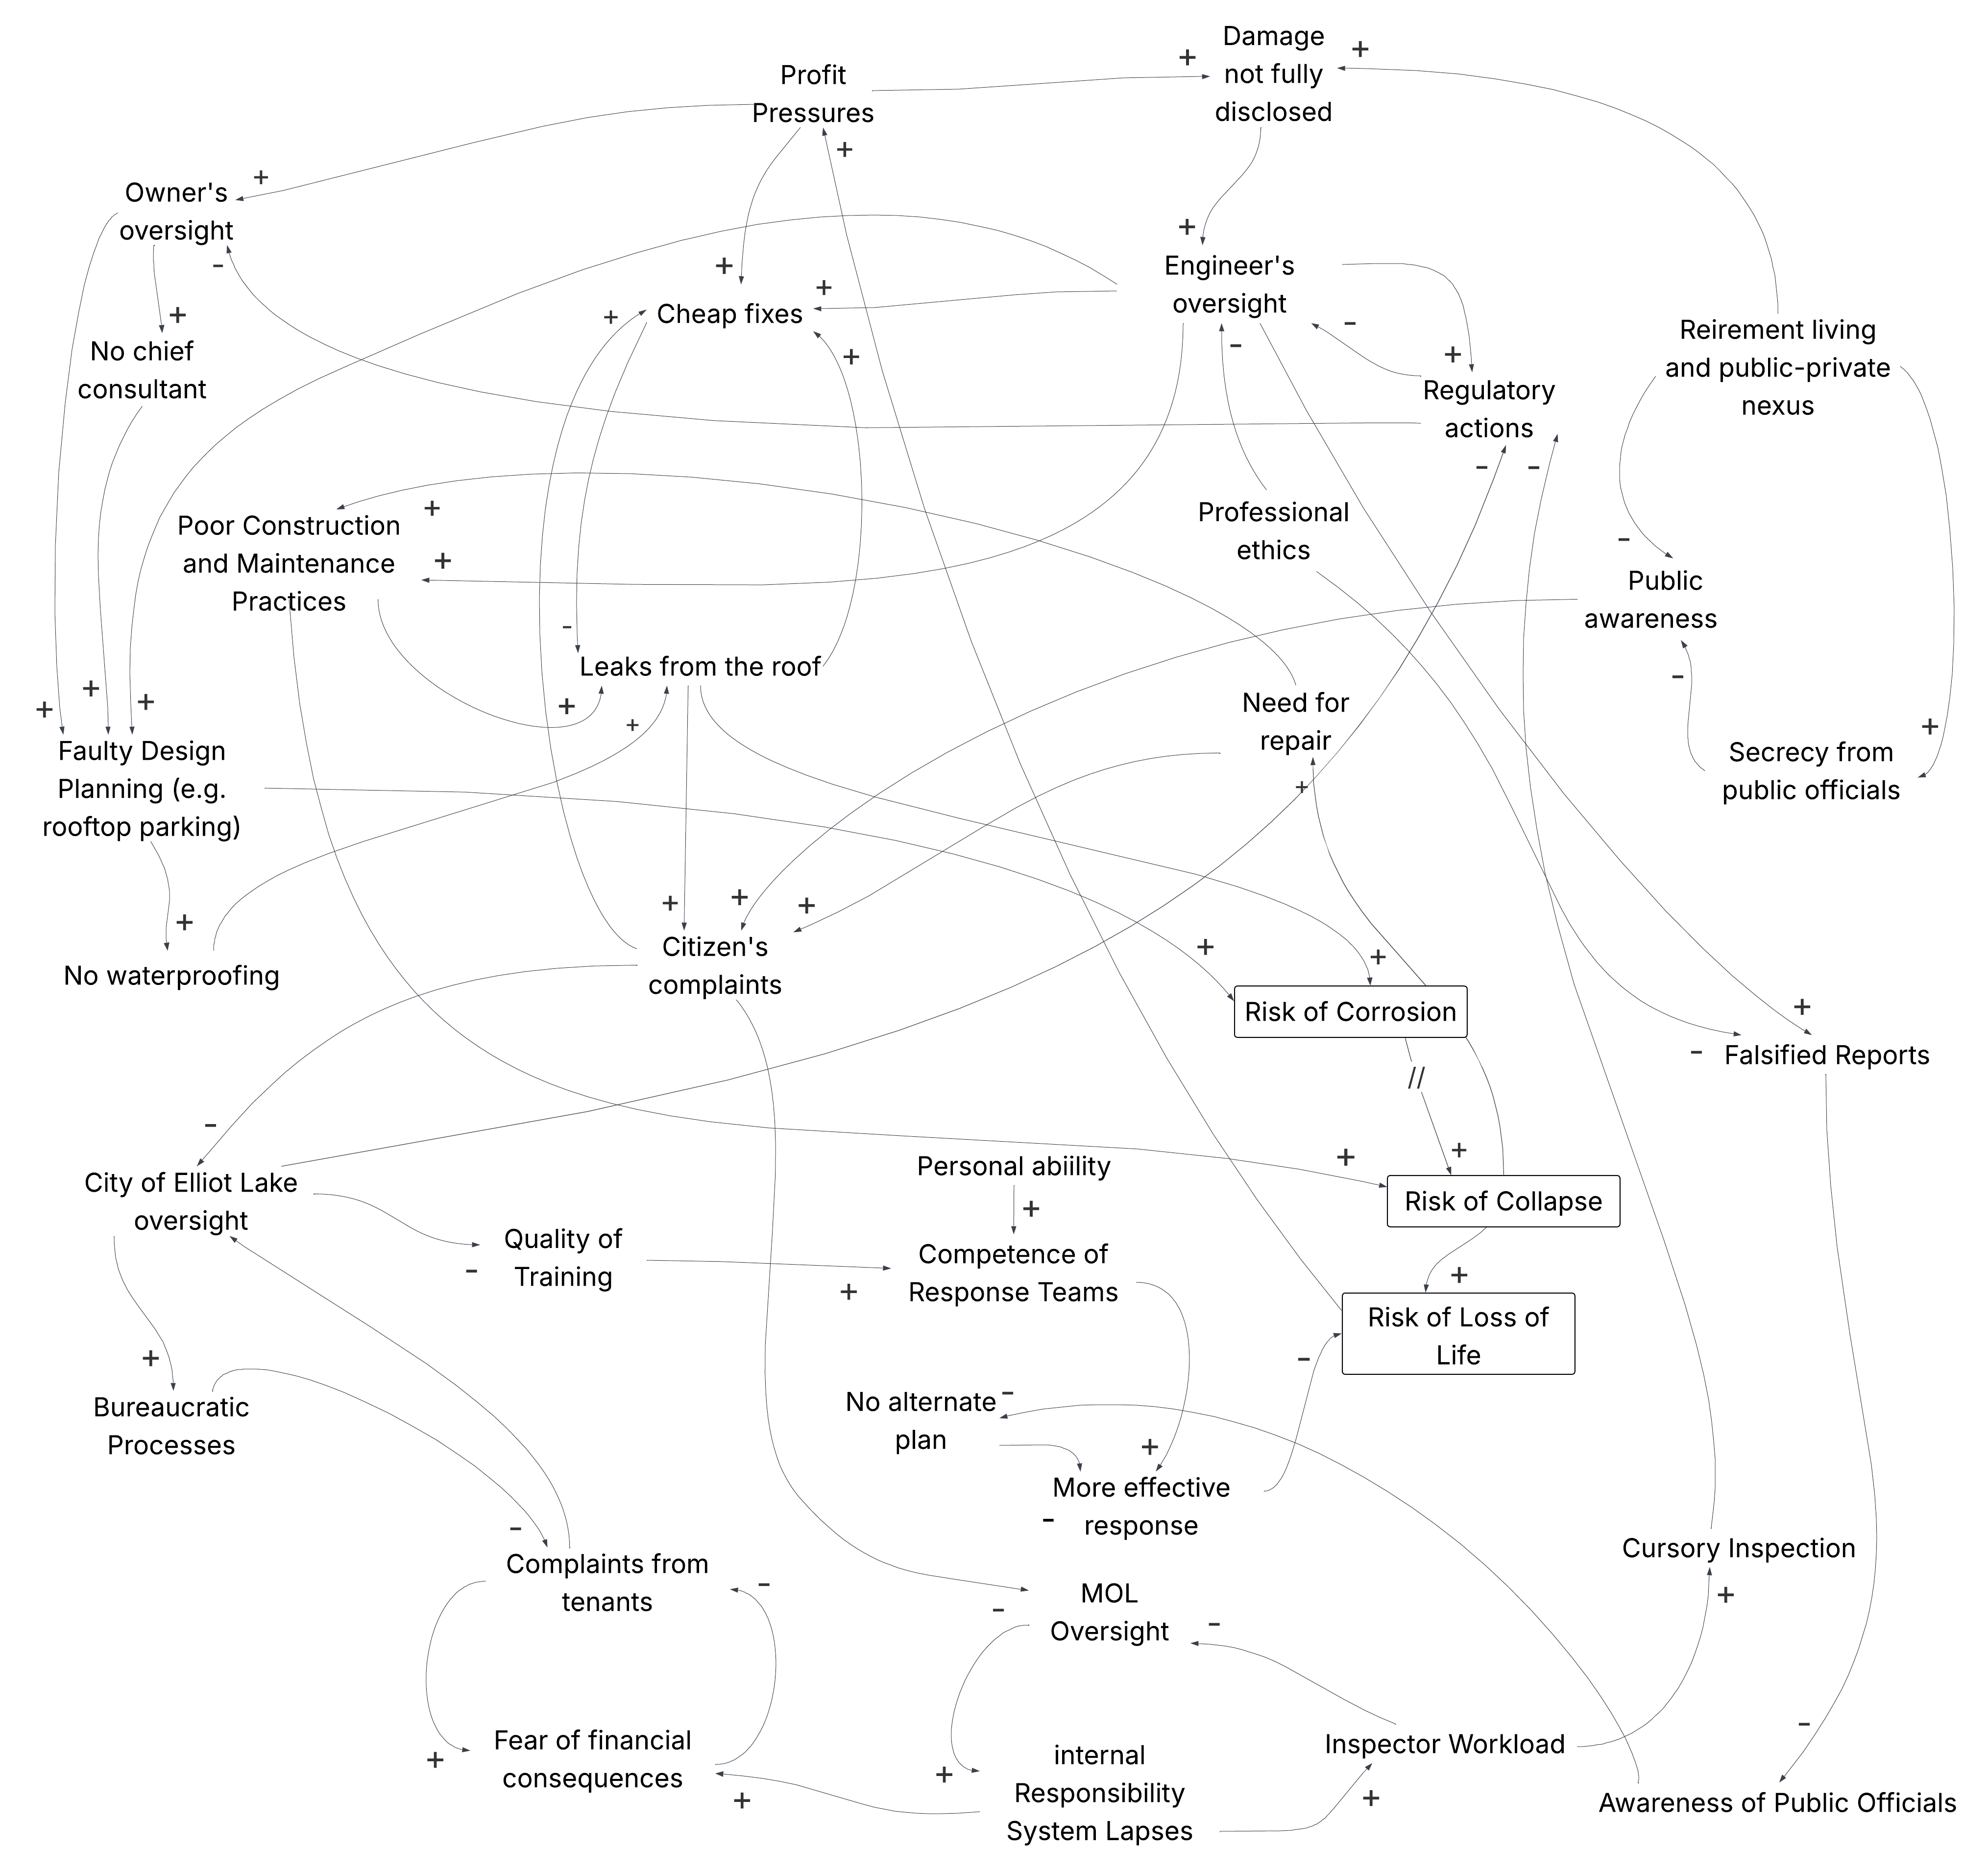
\includegraphics[width=\textwidth]{System Dynamics.png}
    \caption{System Dynamics Model of Algo Centre Mall Collapse}
    \label{fig:sys_dyn}
\end{figure}

In order to arrive at the system dynamic model, the key variables are first identified and then a relationship between them is established using a top-down approach. The previous sections of this report form the basis for this. For example, the risk of corrosion, increases the risk of collapse, which in turn increases the need for repairs, the need for repairs further increases citizens complaints which leads to increasing cheap fixes, which reduces the leaks and reduces the risk of corrosion. Additionally, engineer's oversight increases poor construction and maintenance practices, which increases the risk of collapse, which in turn increases the need for repair. The need for repair increases poor construction and maintenance practices, reinforcing the loop. There are also small balancing loops where engineer's oversight  increases regulatory actions and increase in regulatory actions balance engineer's oversight. Furthermore, there are also factors like personal ability which increase the competence of the response team, that do not form part of a loop. 


\section{CAST Step 6 - Discussion and Recommendations}
% Author: Kecin Li
% Reviewer: Shuhan Zheng

\subsection{Discussion}

The collapse of the Algo Centre Mall was not the result of a single mistake but a culmination of system failures. Although it was the corrosion that caused the gridline G-16 connection to fail, the tragedy would not have taken place without apathy, negligence, and sometimes greed and deception across multiple levels. Safety constraints that could have prevented such a disaster were ineffectively enforced, which revealed a series of systemic flaws in the safety control structure: it relied too heavily on the integrity and judgment of just a few key actors, like the mall owners and their engineers. When these key actors failed to uphold their responsibilities, no robust higher-level controls stepped in. The entire system allowed decades of unchecked deterioration to accumulate and eventually led to the tragedy.

A persistent problem in the Algo Centre Mall's history is the breakdown of feedback loops between stakeholders, partly due to their prioritizing financial considerations over safety. The most notable of such individuals was Bob Nazarian, the final owner of the Algo Centre Mall. Nazarian misrepresented the severity of the mall's structural issues to tenants, municipal officials, and the public, even going so far as to obstruct access to key engineering reports. The Inquiry concluded that he engaged in “subterfuge and falsehood” to delay costly repairs and preserve business operations, despite clear evidence of deterioration. The owners displayed a pattern of using cheap patchwork fixes or even sold the mall when major repairs were needed, and the critical information regarding the mall's actual condition was not passed along. For example, Algocen Realty Holdings never informed Retirement Living of the serious leakage and structural issues documented in engineering reports. This failure to communicate resulted in the new owners and the local government being left unaware of the building's state at the time. 

The inspecting engineers who could have made a difference also failed to act responsibly. In principle, inspections should have acted as an important feedback mechanism; engineers would identify potential hazards and insist on repairs or alert regulators. However, some engineers gave in to client pressure and conflicts of interest rather than to report the truth. Commissioner Bélanger found that certain engineers “forgot the moral and ethical foundation of their vocation” and prioritized business interests over public safety. Investigations revealed that their inspection reports were often written “more with an eye to pleasing clients than [...] warning of potential dangers.” A clear indication of this problem appeared merely weeks before the collapse, when an engineer performed a cursory visual inspection and failed to find or report the severe rusting of a critical connection. Having stemmed from the lack of properly upheld professional standards, this problem further contributed to the failure of communication, which broke down the feedback loops necessary for effective safety management.

Communication breakdowns were also found between the various government and regulatory bodies. Elliot Lake's city council and building department were aware of the mall's chronic leaks and crumbling structure; nevertheless, enforcement actions were slow and weak. Given the Algo Centre Mall's significance to the city's commerce and community, the city officials were reluctant to take strong actions to enforce safety measures, despite complaints from tenants and residents and alike. No penalties or orders for closure were issued throughout the mall's history, and other orders issued by the city fell through without follow-up actions. The Ministry of Labour, which had offices in the mall and conducted numerous inspections, also failed to act on structural safety concerns. The MoL and the City Council acted as separate entities on the same safety matter without coordinating their efforts. They also failed to report the issues and escalate them to higher authorities, displaying a systemic fragmentation between different levels and sectors of government.

Over the decades, the mall's stakeholders also developed a culture of complacency toward its problems. The roof leakage was so persistent that the locals dubbed the building “Algo Falls.” This normalization of the abnormal undermined the sense of urgency that leaks and corrosion should evoke. Minor failures and violations became like a routine. Over time, this cultural adaptation meant that even major warning events (such as a piece of concrete falling or a shopping center owner publicly acknowledging a water leak) did not invoke the appropriate sense of alarm or to prompt immediate action. All parties simply adjusted their expectations in the face of this chronic problem: owners assumed the structure could tolerate ongoing leaks; officials treated complaints as minor maintenance issues rather than imminent hazards; and engineers simply reported “no structural distress” as long as no obvious or major damage was found. In effect, as the abnormal became the norm, the boundary of acceptable risk shifted away from safety limits. The Inquiry observed, “occasional voices of alarm and warning blew by deaf and callous ears.” This condition, therefore, served as a dangerous reinforcing loop and resulted in downplaying the potential risks of buildings.

Meanwhile, inadequate regulatory oversight and enforcement led to a poor design such as the roof of Algo Centre Mall slipping through the building approval process. The 1975 Building Code required that a roof should “shed or drain water effectively” and be watertight. The mall's designer indicated a waterproof layer to be included in the roof design, which satisfied the code requirements. However, the material of the waterproof layer was never specified, and whatever material that was put in place started leaking almost immediately after the mall opened. More critically, Ontario's building regulatory framework had no requirement for periodic structural re-certification or inspection of existing buildings. The only tools available were local property standards bylaws and complaint-driven inspections, and as mentioned earlier, the city's sloppy enforcement rendered these tools inpotent. No systemic feedback loop was in place to ensure proactive inspections of aging buildings by qualified structural engineers on a regular basis. The lack of coordination between enforcement agencies also exacerbated this issue.

In summary, the CAST analysis employed in production of this report revealed that critical lack of communication between different levels of the safety control actors, and the normalization of deviance were the systemic weaknesses that ultimately led to the Algo Centre Mall collapse. 

\subsection{Recommendations}

\subsubsection{Professional Engineers of Ontario (PEO)}
\begin{enumerate}
    \item Ethical Duties: Engineers and architects should be obligated to report any serious safety hazard they encounter, even if it means displeasing a client or employer. Engineers should resist any calls to downplay their findings or delay necessary repairs because their primary duty is to protect public safety. Finally, engineering reports should remain independent and inpartial, and should not be influenced by pressure from clients, politics, and economic factors.
    
    \item More Thorough Inspections and Improved Standards: Structural inspections of existing buildings must a high level of rigor and standardization. Some Key elements should include:
    
    \begin{itemize}
        \item Qualified Inspectors: All critical inspections should be performed by certified professionals and experts in a relevant field. PEO has recommended that inspection reports for existing buildings should be prepared and conducted by a certified structural specialist. This ensures that thorough and accurate inspections.
        
        \item Precisely Defined Scope and Methodology: PEOs should establish clear performance standards that specify the appropriate scope of structural inspections in detail. Different types of structures should have corresponding scopes and inspection procedures. For example, if an engineer is only retained to inspect the roof, their engienering reports should not give the impression that the inspection has covered the whole building. Additionally, the inspection guidelines should also outline the bounds of a “visual inspection” (e.g. visual inspection of the surfaces exposed to public vs. removaling ceiling tiles and insulation materials to inspect structural elements behind them) and inspections where more thorough methods (like removing finishes or taking material samples) are required.

        \item Documentation and evidence: Inspection reports should be rigorous and properly documents corresponding evidence. This is to ensure that both the engineer and the client cannot temper with the report's content. For example, if the report mentions that a specific building structure or component is corroded, corresponding photos must be provided. Data indicators should also be standardized to enable cross-references with the inspection findings as well as the analysis of failures.

        \item Clear Warnings and Follow-up: If applicable, the engineer's report should include explicit warnings about the risks from the discovered issues, and the concequences of neglecting them. The communciation with client must be clear and precise, ensuring that the client fully awares of the extent of the issues, and that the engineer's recommendations are properly and accurately conveyed to them.
    \end{itemize}
    
    \item Mandatory Continuing Education and Specialization: The engineering profession must ensure that its members keep their skills and knowledge up to date. 
    
    Regular training conducted by engineering organizations should cover topics including the current methods of detecting structural deterioration, engineering ethics, in addition to case studies of failures (such as Algo Mall). PEO offeres a Designated Structural Engineer certification for those who with advanced experiences in structural engineering. Inspections by these specialists should be required by law for complex or high-risk structures.

\end{enumerate}

\subsubsection{Ministry of Municipal Affairs and Housing (MMAH)}
\begin{enumerate}
    \item Mandatory and Regular Structural Inspections: Structural inspections must be strictly enforced and conducted regularly. All large or aging buildings that are open to the public should undergo thorough structural inspections by qualified engineers on a regular basis. These reports would point out any signs of building code violation at the time of inspection (if any is present), and these reports must be submitted to local authorities to create a law-binding record.

    \item Adequate Financial Planning for Maintenance: Owners often defer maintenance due to cost. The Ontario provincial government could implement policies to encourage or require owners to set aside funds for capital repairs. This funding could be adjusted based on the building's size, age, and condition at the last inspection.

    \item Timely Action on Inspection Findings: The local municipality should enact rules that require property owners to bring their buildings into compliance with the Ontario Building Code within a reasonable time frame after an inspection. If an owner fails to act, the municipality should have the authority to intervene and perform the necessary emergency work, billing the owner for the costs incurred. This would ensure that public safety is not compromised by the financial difficulties of property owners.
    
    \item Structural Complaint Hotline: A municipal building safety hotline should be put in place and be made aware by buildign staff tenants, or visitors and alike. An alternative to the hotline could also be implemented on a case-by-case basis. A clear line of communication should be available for reporting issues that directly affect the safety of the building.
    
    Each complaint must be logged and linked to the building's file once it has been confirmed. If the municipal Building Department fails to act within a defined period, the complaint should automatically be escalated to the MMAH for review and possible further investigation.
\end{enumerate}

\subsubsection{Ontario Building Code Commission (OBCC)}

\begin{enumerate}
    \item Empowering Building Officials: OBCC should empower local building officials while preventing abuse of power and corruption, giving them the power to intervene when safety hazards are identified during inspections. In practice, this could allow Chief Building Officials (CBOs) to require preventive repairs or further expert assessments if an inspection report indicates potential structural issues. 
    
    \item Independent Structural Audit Panels: OBCC should establish independent audit panels for high-risk buildings, with the goal of verifying and validating the findings of regular inspectors. These panels would conduct reviews of engineering reports and their corresponding sites on a regular or random basis, ensuring that the inspections are thorough and that the findings are accurate.
\end{enumerate}


\subsubsection{Ministry of Labour, Immigration, Training and Skills Development}
\begin{enumerate}
    \item Whistleblower protections: The Ontario provincial government could introduce whistleblower protections for certain professionals. If engineers report safety issues to the authorities when the owner is irresponsible or unresponsive, they should be protected from legal or professional repercussions. This encourages professionals to act in the public interest first and foremost.
\end{enumerate}


\subsubsection{Ministry of Public and Business Service Delivery and Procurement (MPBSDP) - formerly Ministry of Government and Consumer Services (MGCS)}
\begin{enumerate}
    \item No Sale as a Safety Loophole: (With necessary support from MMAH) All known critical structural issues must be solved or at least transparently disclosed before a ownership transfer. The process of transferring ownership of a property should involve a new inspection afforded by the seller so that the new owner cannot claim ignorance. Essentially, unless explicitly stated, previous owners of a property should be held liable for any damages to the property that were not disclosed to the new owner.

    \item Post-Incident Disclosure Protocols: When serious structural failure or collapse occurs, detailed engineering findings must be summarized and shared in a post-incident disclosure document. MPBSD should be required to disclose causes, decision errors, and systemic failures in a straightforward language. These summaries should be reviewed by the PEO and the Office of Building Codes Commissioners (OBCC) to ensure that technical and code-related findings are widely shared. This record will be useful for long-term learning and inform future policy development.

\end{enumerate}

% Design and Maintenance: Suggest improvements in building design practices and maintenance protocols to prevent similar failures. TERESA

% Regulatory Reforms: Propose changes to regulatory frameworks to enhance oversight and enforcement of safety standards. KEVIN

% Organizational Changes: Recommend organizational reforms to improve communication, accountability, and safety culture among stakeholders. RAUL

\section{Aftermath}
%TERESA

\section{Conclusion}
% Summary of Findings: Recap the key insights gained from the CAST analysis.

% Implications for Future Practice: Discuss how these findings can inform future practices in building design, maintenance, and regulation.

\section*{Appendices}

\newpage
\printbibliography
\end{document}
